% ===========================
% 2026.03.16
% --------------
% Collaborative Computing Lab
% Hongik University
% Hosung.Kim
% ==============

% This is samplepaper.tex, a sample chapter demonstrating the
% LLNCS macro package for Springer Computer Science proceedings;
% Version 2.21 of 2022/01/12
%
\documentclass[runningheads]{llncs}
%
\usepackage[T1]{fontenc}
% T1 fonts will be used to generate the final print and online PDFs,
% so please use T1 fonts in your manuscript whenever possible.
% Other font encondings may result in incorrect characters.
%
\usepackage{graphicx}
% Used for displaying a sample figure. If possible, figure files should
% be included in EPS format.
%
% If you use the hyperref package, please uncomment the following two lines
% to display URLs in blue roman font according to Springer's eBook style:
%\usepackage{color}
%\renewcommand\UrlFont{\color{blue}\rmfamily}
%\urlstyle{rm}
%

%Hosung.Kim
\usepackage{booktabs}%

\begin{document}
%
\title{Live Mobile Learning System with User-Adjustable UI}
%
%\titlerunning{Abbreviated paper title}
% If the paper title is too long for the running head, you can set
% an abbreviated paper title here
%
\author{First Author\inst{1}\orcidID{0009-0001-2694-0805} \and
Second Author\inst{2}\orcidID{1111-2222-3333-4444}}
% \author{Ho Sung Kim\inst{1}\orcidID{0009-0001-2694-0805} \and Jang Ho Lee\inst{2}\orcidID{1111-2222-3333-4444}}
%
\authorrunning{F. Author et al.}
% \authorrunning{H. S. Kim and J. H. Lee}
%
% First names are abbreviated in the running head.
% If there are more than two authors, 'et al.' is used.
%
\institute{Department of Computer Engineering, Hongik University, Seoul, Korea
\email{hosungkim5108@gmail.com} \and
Springer Heidelberg, Tiergartenstr. 17, 69121 Heidelberg, Germany
\email{lncs@springer.com}}
%
\maketitle              % typeset the header of the contribution
%
\begin{abstract}
Most existing live mobile distance learning systems do not display presentation slides and a whiteboard simultaneously, resulting in a discrepancy from a real classroom where both can be viewed together. Even when both are displayed simultaneously, the limited screen size of mobile devices can significantly compromise their visibility, negatively affecting both instructor's usability and students' comprehension. Therefore, we propose a live mobile distance learning system with a user-adjustable UI that allows instructors to dynamically resize the slides and whiteboard areas. This system allows students to maintain sufficient visibility on limited screen sizes, providing an experience closer to that of a real classroom. The results of our preliminary evaluation show that the proposed system outperforms existing systems in visibility and comprehensibility, demonstrating that a user-adjustable UI can effectively enhance learning performance in mobile remote education environments.

\keywords{Live mobile learning \and Whiteboard \and Annotation}
\end{abstract}
%
%
%
\section{Introduction}
Distance learning has long been studied as a means of enabling students to attend classes without physically presence. With the widespread use of mobile devices, mobile learning has attracted significant attention from researchers, allowing students to participate in a learning session anytime and anywhere using smartphones or tablets\cite{10.1145/1414558.1414568}.

Early mobile learning systems include Classroom Presenter\cite{ClassroomPresenter} and MLVLS\cite{MLVLS}. Classroom Presenter, a tablet-based live mobile learning system, supports slides sharing with annotation but lacks video and chat features for interaction between a teacher and students. MLVLS, running on Symbian smartphones, did include video, but interaction remains limited, and small screens make it difficult to read detailed slides.

The COVID-19 pandemic dramatically accelerated the adoption of distance learning systems, as distance learning became the only viable alternative to the traditional face-to-face classroom. Since then, live mobile learning has evolved beyond a temporary backup plan into a new standard in education. During the pandemic, video conferencing platforms such as Cisco Webex\cite{Webex}, Zoom\cite{Zoom}, Microsoft Teams\cite{MicrosoftTeams}, Google Meet\cite{GoogleMeet} were widely used for distance learning. These platforms support various features, including slides with annotation, whiteboard, instructor video, chat, and participant management. However, they do not support the simultaneous view of both presentation slides and a whiteboard. Although a simple side-by-side layout is possible, the limited screen size of mobile devices can significantly compromise their visibility. It negatively affects both the instructor's delivery and the students' overall comprehension.

To address this limitation, the Large-Sized Tablet-Based Live Mobile Learning System\cite{10.1007/978-3-030-88207-5_24} was proposed. By leveraging the larger display area of tablets, this system enables the simultaneous view of slides and a whiteboard and supports features such as slides with annotation, whiteboard, instructor video, chat, and participant management. 이 시스템은 in terms of lecture understanding, sophistication of a lecture, and the feedback to a question에서 더 효과적임이 검증되었다.

To extend the benefits of the Large-Sized Tablet-Based Live Mobile Learning System, which have been validated on large-sized tablets, to a wider range of general mobile devices, we propose a live mobile learning system with a user-adjustable UI which allows instructors to dynamically resize the slide and whiteboard areas. This flexible layout ensures that complex slides remain sufficiently legible even on compact displays, thereby delivering a learning experience that more closely approximates the effectiveness and interactivity of  a traditional classrooms.

\section{Live Mobile Learning System with User-Adjustable UI}

Figure~\ref{fig1} shows the run-time communication architecture of the proposed system.

\begin{figure}
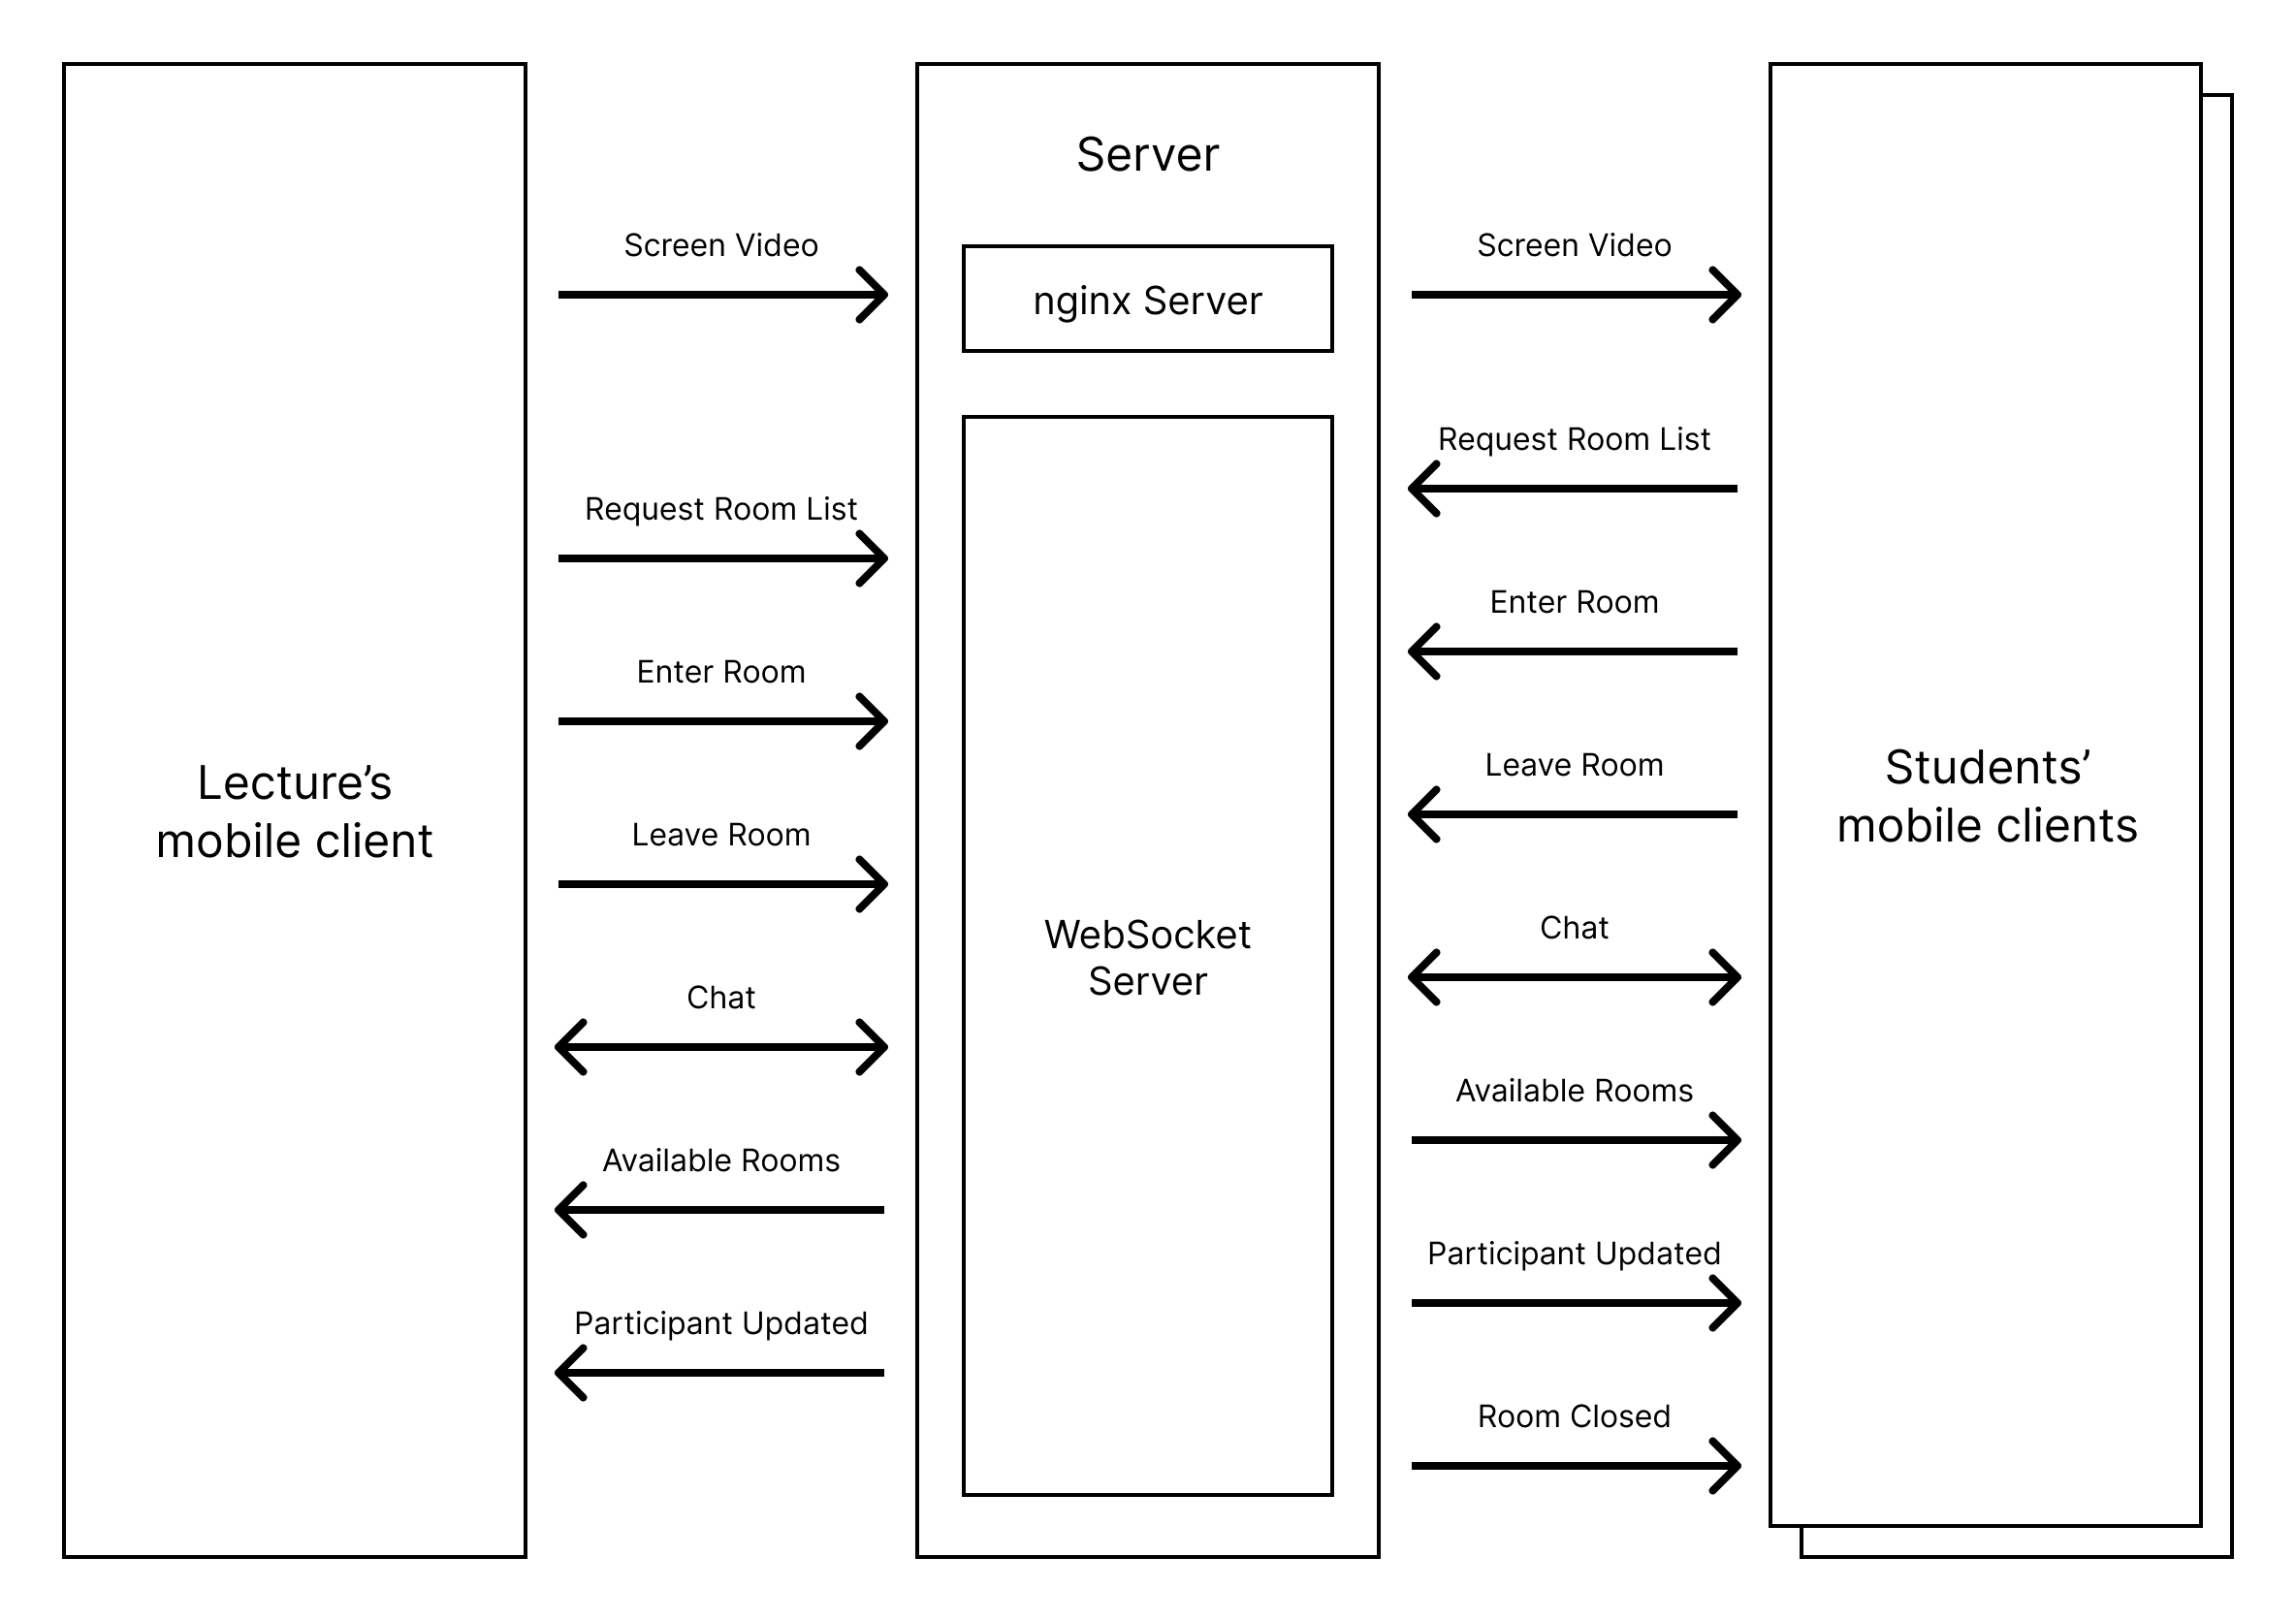
\includegraphics[width=\textwidth]{fig1.png}
\caption{Communication architecture of the proposed system} \label{fig1}
\end{figure}

% The system consists of a server and clients. 서버는 NGINX 서버와 WebSocket 서버로 이루어져있다. NGINX 서버는 RTMP(Real-Time Messaging Protocol)에 의해 강사측 모바일 클라이언트로부터 슬라이드, 주석, 화이트보드, 강사 캠 영상, 음성이 포함된 영상을 받아서 학생측 모바일 클라이언트에게 전달한다. WebSocket서버는 강의실 생성, 입장 및 퇴장, 강의실 종료, 강의실 목록 조회, 참여자 명단 동기화 등 강의실 관리 기능과 채팅 기능을 담당한다. 두 서버는 macOS 환경에서 Xcode Command Line Tool로 통합되어 하나의 Xcode Target으로 실행된다.
The system consists of a server and multiple clients. The server is composed of an NGINX server and a WebSocket server. The NGINX server multicasts receives a stream—including lecture slides, annotations, whiteboard content, instructor camera video, and audio—from the instructor’s mobile client via the RTMP (Real-Time Messaging Protocol), and delivers it to student clients in real time. The WebSocket server handles classroom management functionalities, including room creation, entry and exit, room termination, room list retrieval, participant synchronization, and chat. Both servers are integrated and executed as a single Xcode target using Xcode Command Line Tools in a macOS environment, allowing unified deployment and management.

% 스트리밍 서버는 서버 실행 시 \verb+Process()+를 통해 nginx.exe 실행파일과 nginx.conf 설정파일을 프로그램적으로 호출하여 자동으로 실행되며, 종료 시에도 동일한 방식으로 제어된다. 이를 통해 운영자는 별도의 명령 입력 없이 안정적으로 서버를 일원화하여 관리할 수 있다.
The streaming server is automatically launched when the server starts by programmatically executing the nginx binary and configuration file using \verb+Process()+. It is also terminated in the same manner. This approach enables stable and centralized server management without requiring manual command-line operations.

%% WebSocket 서버는 Swift Network Framework\cite{Network}의 \verb+NWProtocolWebSocket+을 기반으로 구현되었으며, 강의실 생성·종료·입장·퇴장, 강의실 목록 조회, 참여자 명단 동기화 등 다중 강의실 기능과 채팅 기능을 제공한다. 이처럼 다양한 기능을 제공하기 위해 서버-클라이언트 간 통신에는 \verb+Codable+을 상속한 \verb+enum+을 사용하여 기능 확장을 용이하게 하고 다양한 종류의 메세지를 주고받을 수 있도록 하였다.
%The WebSocket server is implemented using \verb+NWProtocolWebSocket+ from the Apple Network Framework\cite{Network}. It supports multi-room functionality and chat by handling events such as room creation, termination, entry, exit, room list updates, and participant synchronization. To efficiently support various message types and ensure extensibility, communication between the server and clients is designed using a \verb+Codable+-based \verb+enum+, allowing structured and scalable message handling.
%
%% WebSocket 서버는 모든 강의실을 UUID를 키로 하는 딕셔너리 형태로 관리한다. 강의실 목록이 변경되면 Available Room 메세지를 모든 클라이언트에게 브로드캐스트한다. Enter Room 또는 Leave Room 메세지를 수신하면 해당 클라이언트를 관련 강의실에 등록하거나 제거한다. 강의자가 퇴장하면 해당 강의실의 모든 학생에게 Room Closed 메세지를 전송하여 강의 종료를 알린다. 참여자 명단 변경이나 채팅 메세지 수신 시, 해당 강의실의 모든 클라이언트에게 각각 Participant Updated 메세지 또는 채팅 메세지를 동일 강의실 내 모든 클라이언트에게 브로드캐스트한다.
%The WebSocket server manages all classrooms using a dictionary with UUID keys. When the room list changes, an Available Room message is broadcast to all clients. Upon receiving Enter Room or Leave Room messages, the server registers or removes the client from the corresponding room. When an instructor leaves, a Room Closed message is broadcast to all participants in the room. Similarly, participant updates and chat messages are broadcast only to clients within the same room.
%
%% 그림\ref{fig3}은 홈화면을 보여준다. 홈화면에서는 강의실 목록들 중 하나를 선택하여 학생으로 입장하거나 우측 하단의 +버튼을 눌러 강의실을 새로 생성하여 강사로 수업을 시작할 수 있다. 강의실 목록은 WebSocket 서버와의 통신을 통해 실시간으로 갱신되며, 강의실 명단 \verb+UITableView+를 아래로 스크롤하여 수동으로 새로고침할 수도 있다. 강의실 입장과 생성 이벤트는 Enter Room 메세지를 WebSocket 서버에 전송하여 처리된다.
%Figure~\ref{fig3} shows the home screen of the application. Users can either join an existing classroom as a student or create a new room using the "+" button to start a lecture as an instructor. The room list is updated in real time via communication with the WebSocket server, and users can also manually refresh the list by pulling down the \verb+UITableView+. Both room creation and entry are handled by sending an Enter Room message to the server.
%
%\begin{figure}
%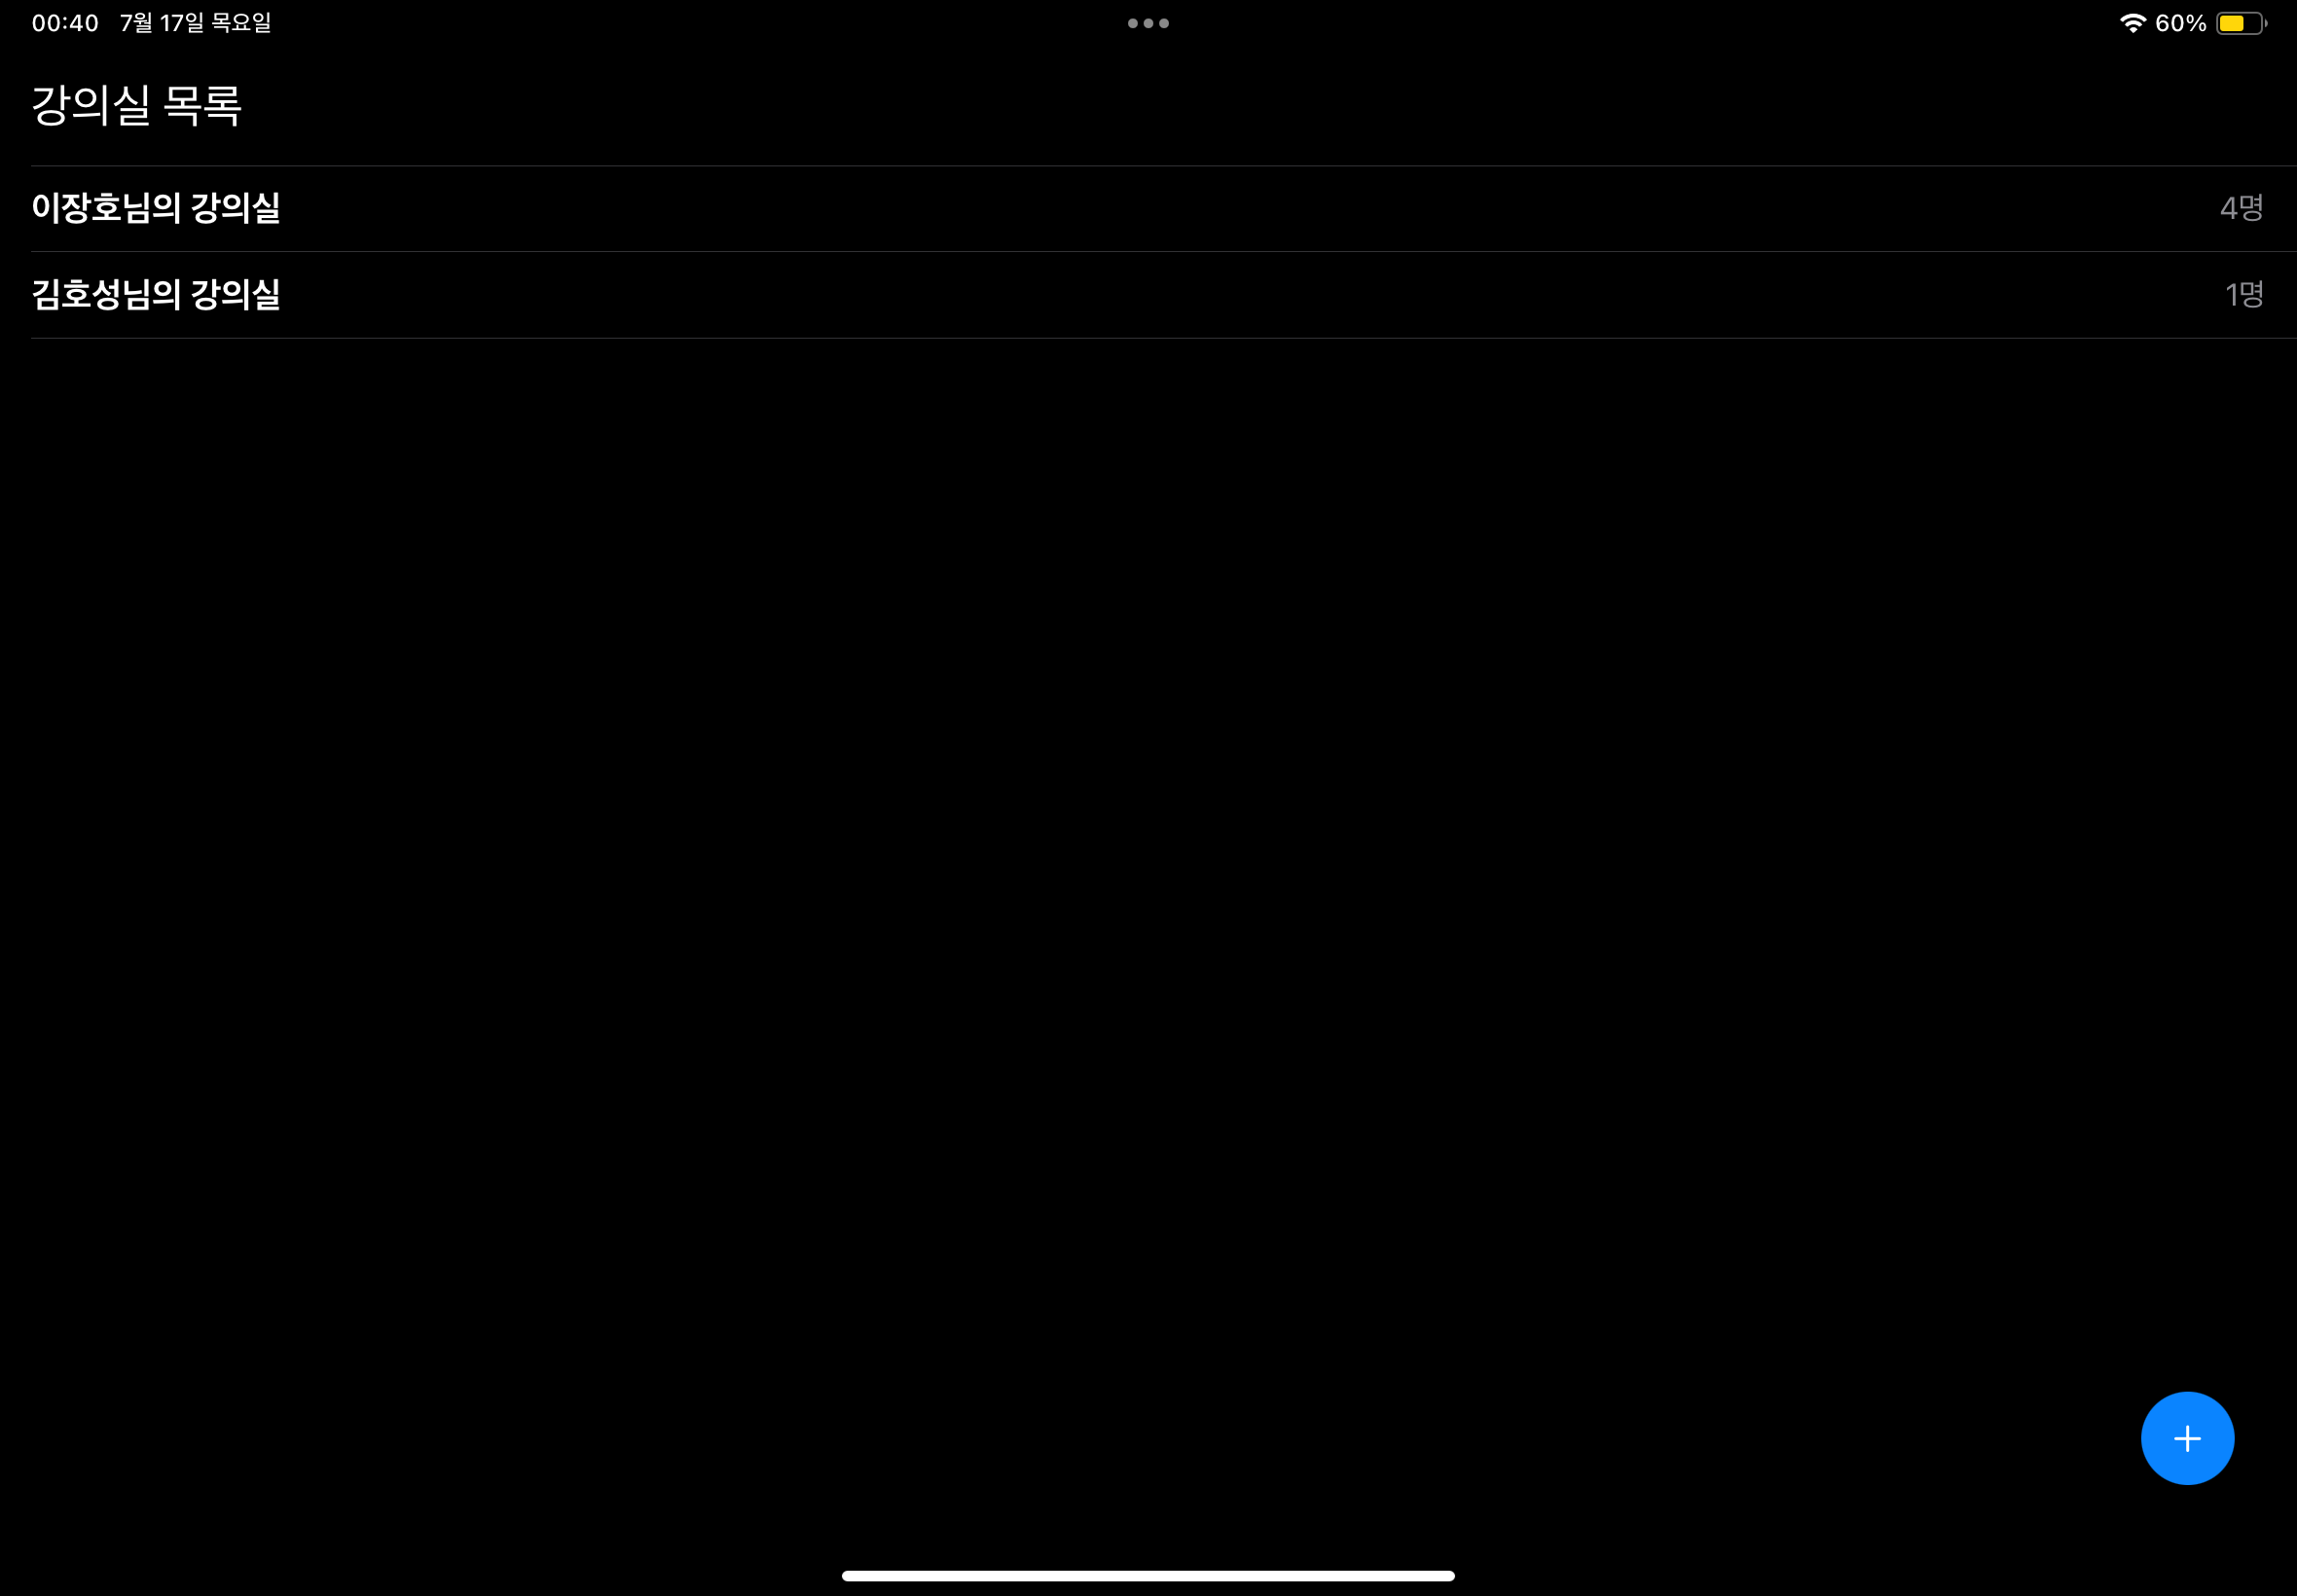
\includegraphics[width=\textwidth]{fig3.png}
%\caption{User interface of a home screen} \label{fig3}
%\end{figure}
%
%% 그림\ref{fig4}는 강사측 클라이언트의 강의실화면을 보여준다. 해당 화면의 UI는 PDF 강의 슬라이드, 화이트보드, 강사 카메라 영상, 참여자 명단, 채팅창 등으로 구성된다. 각 요소에 대한 자세한 설명은 다음과 같다.
%\noindent
%Figure~\ref{fig4} shows the instructor-side classroom interface. The UI consists of lecture slides (PDF), a whiteboard, instructor camera video, a participant list, and a chat panel. Detailed descriptions of each component are as follows.
%
%\begin{figure}
%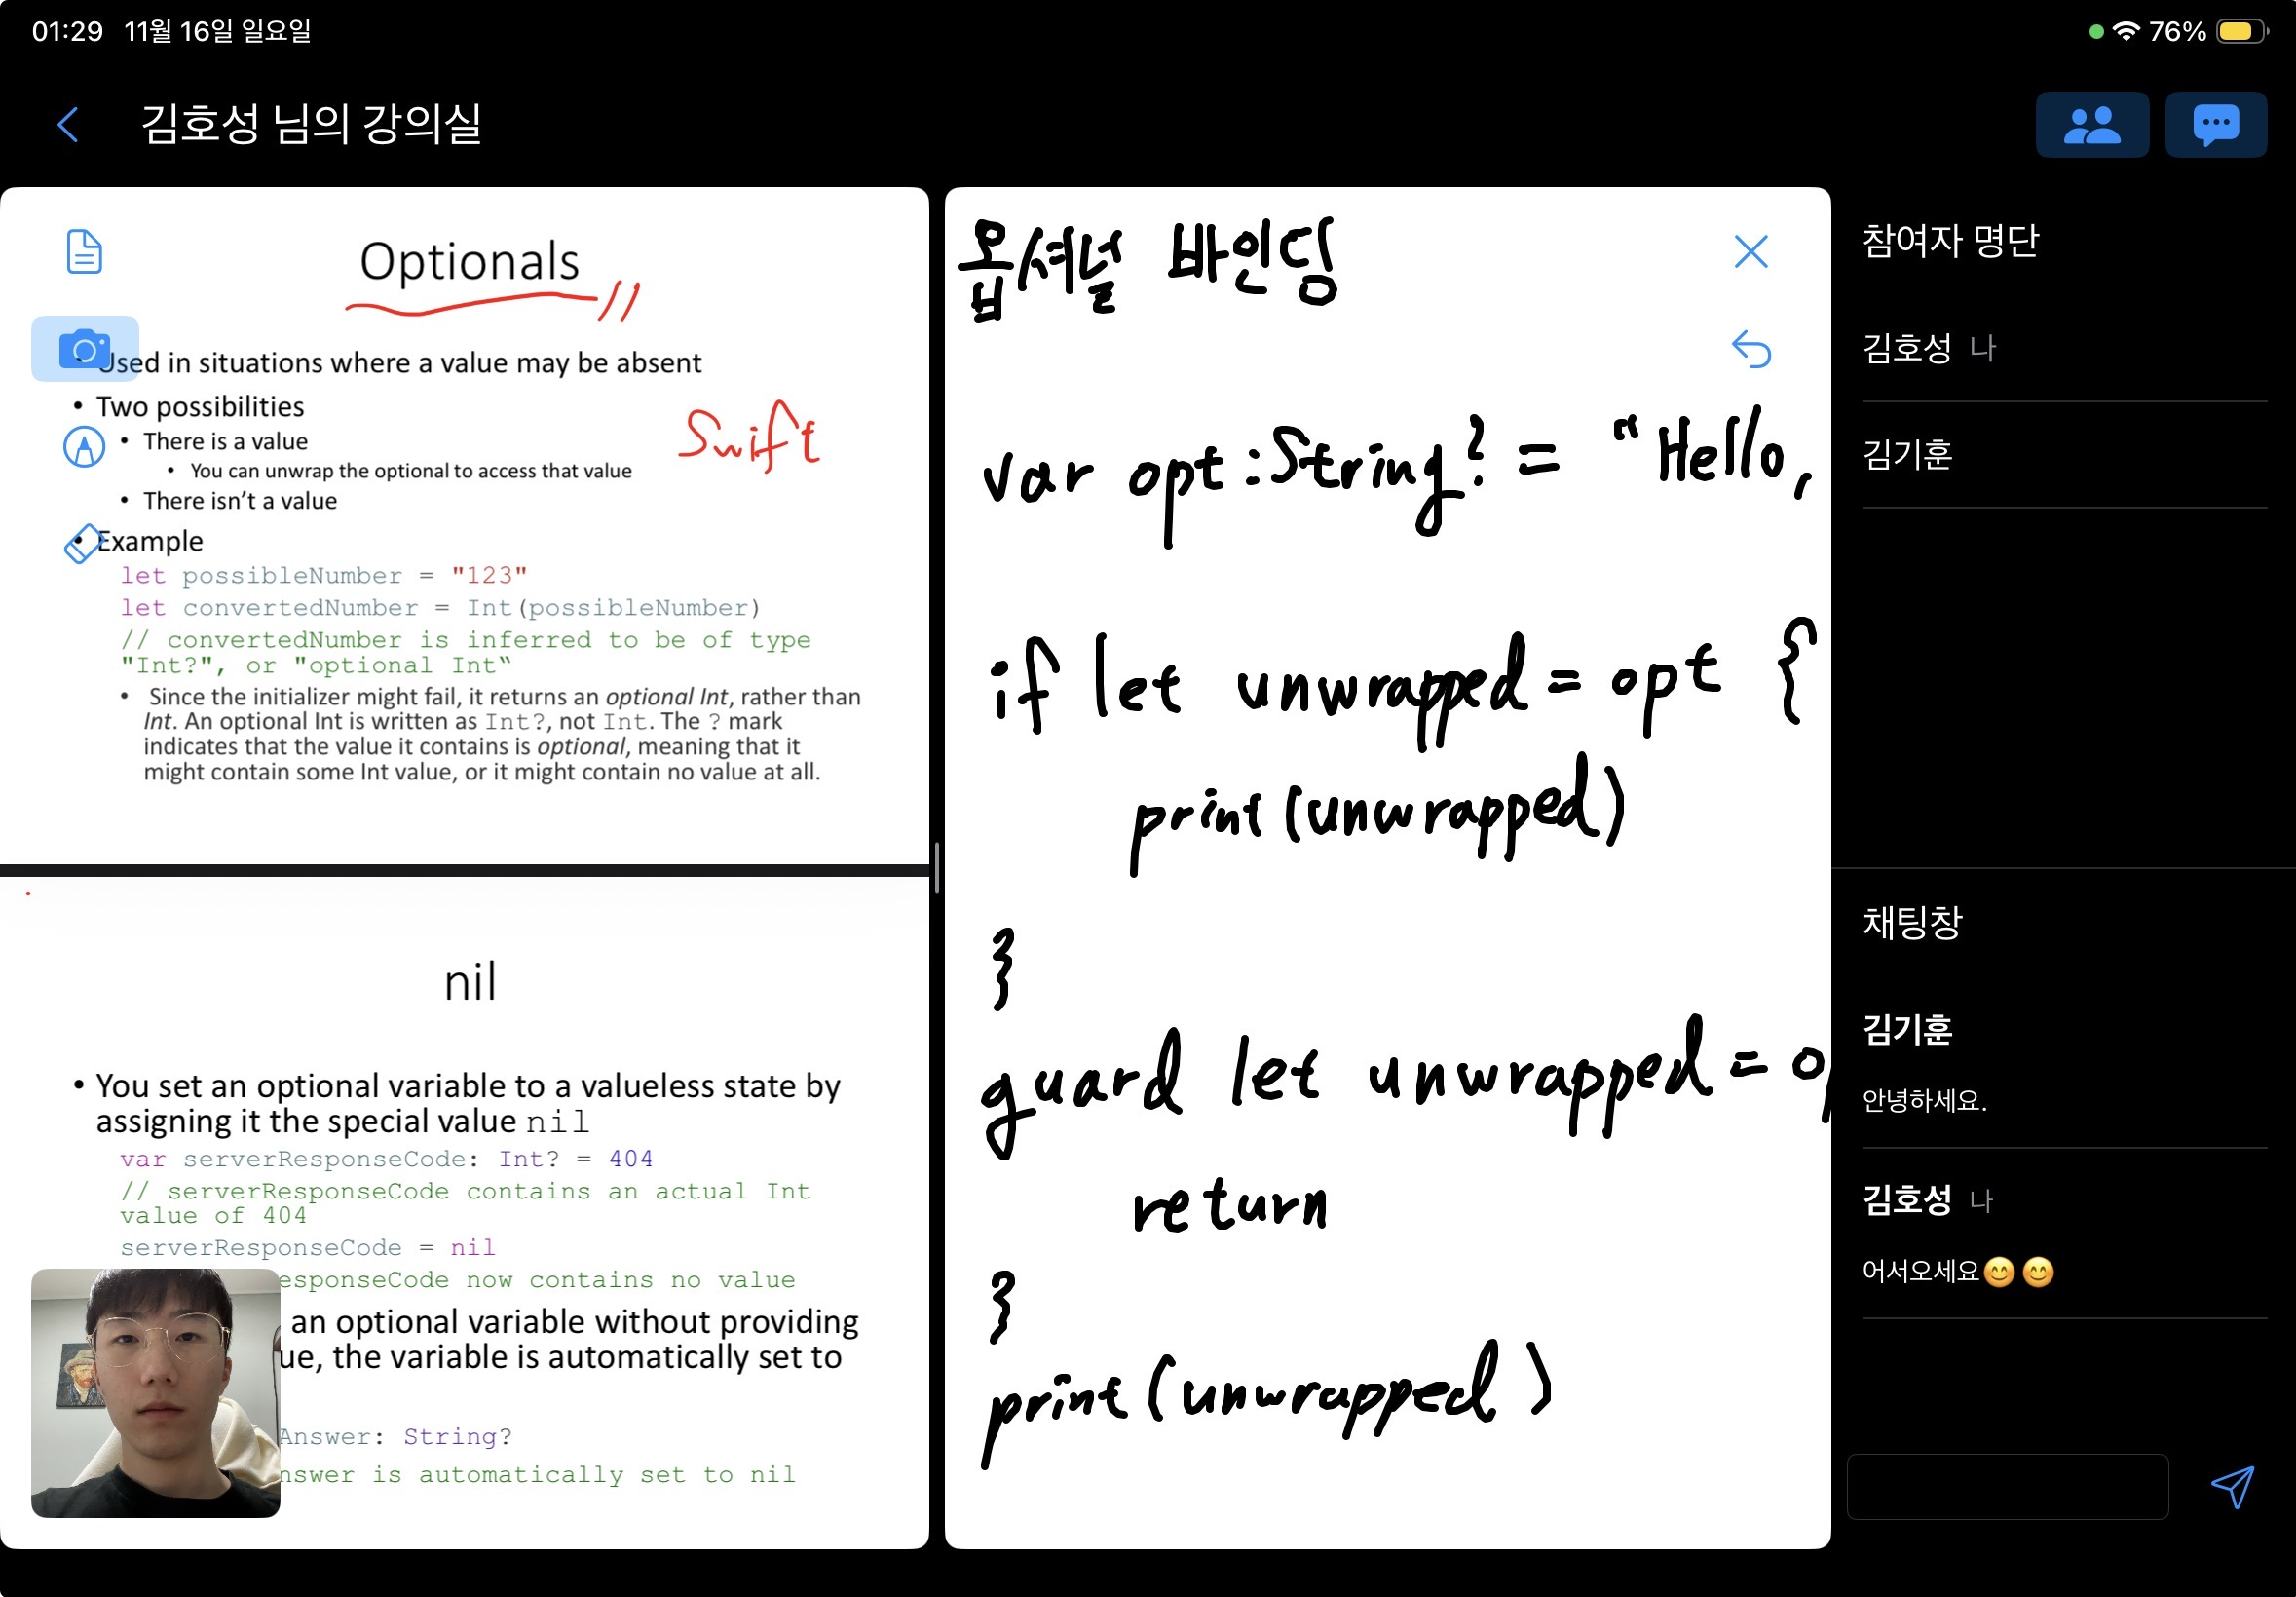
\includegraphics[width=\textwidth]{fig4.jpg}
%\caption{User interface of a classroom screen} \label{fig4}
%\end{figure}
%
%% PDF 강의 슬라이드는 Apple Framework인 PDFKit\cite{PDFKit}의 \verb+PDFView+를 사용하여 구현되었다. 좌측 상단 문서 모양 버튼을 누르면 \verb+UIDocumentPickerViewController+를 통해 기기에 저장된 PDF 파일을 선택할 수 있고 선택된 파일의 링크를 가져와서 \verb+PDFView+로 화면에 출력한다.
%\noindent
%Lecture slides are implemented using \verb+PDFView+ from PDFKit\cite{PDFKit}. Instructors can select a PDF file stored on the device via \verb+UIDocumentPickerViewController+, and the selected file is rendered using \verb+PDFView+.
%
%% 강의 슬라이드의 주석 기능은 PDFKit의 \verb+PDFPageOverlayViewProvider+를 사용하여 각 \verb+PDFPage+의 \verb+overlayView+에 PencilKit\cite{PencilKit}의 \verb+PKCanvasView+를 추가하여 구현하였다. 좌측 상단의 펜 버튼과 지우개 버튼은 토글식으로 구현되어서 선택되어있는 버튼에 따라 \verb+PKTool+을 펜 또는 지우개로 설정한다. 둘 다 비활성화된 상태일 때는 PDF 문서 스크롤로 작동한다.
%Annotation on slides is implemented using \verb+PDFPageOverlayViewProvider+, where a \verb+PKCanvasView+ from PencilKit\cite{PencilKit} is added to the \verb+overlayView+ of each \verb+PDFPage+. Pen and eraser tools are implemented as toggle buttons, which switch the \verb+PKTool+ accordingly. When both tools are disabled, the view behaves as a scrollable PDF document.
%
%% 화이트보드는 사용자의 터치 이벤트를 직접 감지하여 선을 그리는 방식으로 구현하였다. 터치 이벤트를 \verb+override+하여 사용자가 화면을 터치하면 \verb+touchesBegan+에서 새로운 \verb+UIBezierPath+ 객체를 생성하고 배열에 저장하며, 터치 이동 시에는 \verb+touchesMoved+에서 해당 객체에 좌표를 추가하고 \verb+setNeedsDisplay()+를 호출하여 화면을 갱신하였다. 저장된 \verb+UIBezierPath+들은 \verb+override+한 \verb+draw+ 함수에서 그려진다. 우측 상단 버튼들을 통해 undo와 clear 기능도 지원한다.
%The whiteboard is implemented by directly handling touch events. A new \verb+UIBezierPath+ is created in \verb+touchesBegan+ and stored in an array. As the user moves their finger, points are appended in \verb+touchesMoved+, and \verb+setNeedsDisplay()+ is called to update the view. All stored paths are rendered in the overridden \verb+draw+ method. Undo and clear functionalities are also provided.
%
%% 강사의 전면 카메라의 영상은 \verb+AVCaptureVideoPreviewLayer+를 기반으로 구현한 \verb+CameraPreviewView+를 통해 제공된다. \verb+CameraPreviewView+는 \verb+UIView+를 상속하며, \verb+layerClass+를 \verb+AVCaptureVideoPreviewLayer+로 지정하여 \verb+AVCaptureSession+을 통해 전면 카메라 영상을 실시간으로 렌더링하여 강의자가 자신의 영상 상태를 직접 확인할 수 있도록 하였다.
%The instructor’s front camera is displayed using a custom \verb+CameraPreviewView+ based on \verb+AVCaptureVideoPreviewLayer+. This view subclasses \verb+UIView+ and overrides \verb+layerClass+ to render real-time camera input via an \verb+AVCaptureSession+, allowing the instructor to monitor their own video.
%
%% 그림\ref{fig4}, \ref{fig5}, \ref{fig6}과 같이 참여자 목록과 채팅창은 접이식 구조로 구현하여 불필요한 화면 점유를 최소화하였다. 두 구성요소는 \verb+UIStackView+에 포함되어 있으며, 우측 상단 각각의 토글 버튼에 따라 \verb+isHidden+ 속성을 조정함으로써 열고 닫을 수 있도록 구현하였다.
%As shown in Figures~\ref{fig4}, ~\ref{fig5}, and ~\ref{fig6}, the participant list and chat panel are implemented as collapsible UI components to minimize unnecessary screen usage. These components are embedded in a \verb+UIStackView+, and their visibility is controlled by toggling the \verb+isHidden+ property via corresponding buttons.
%
%\begin{figure}[H]
%\centering
%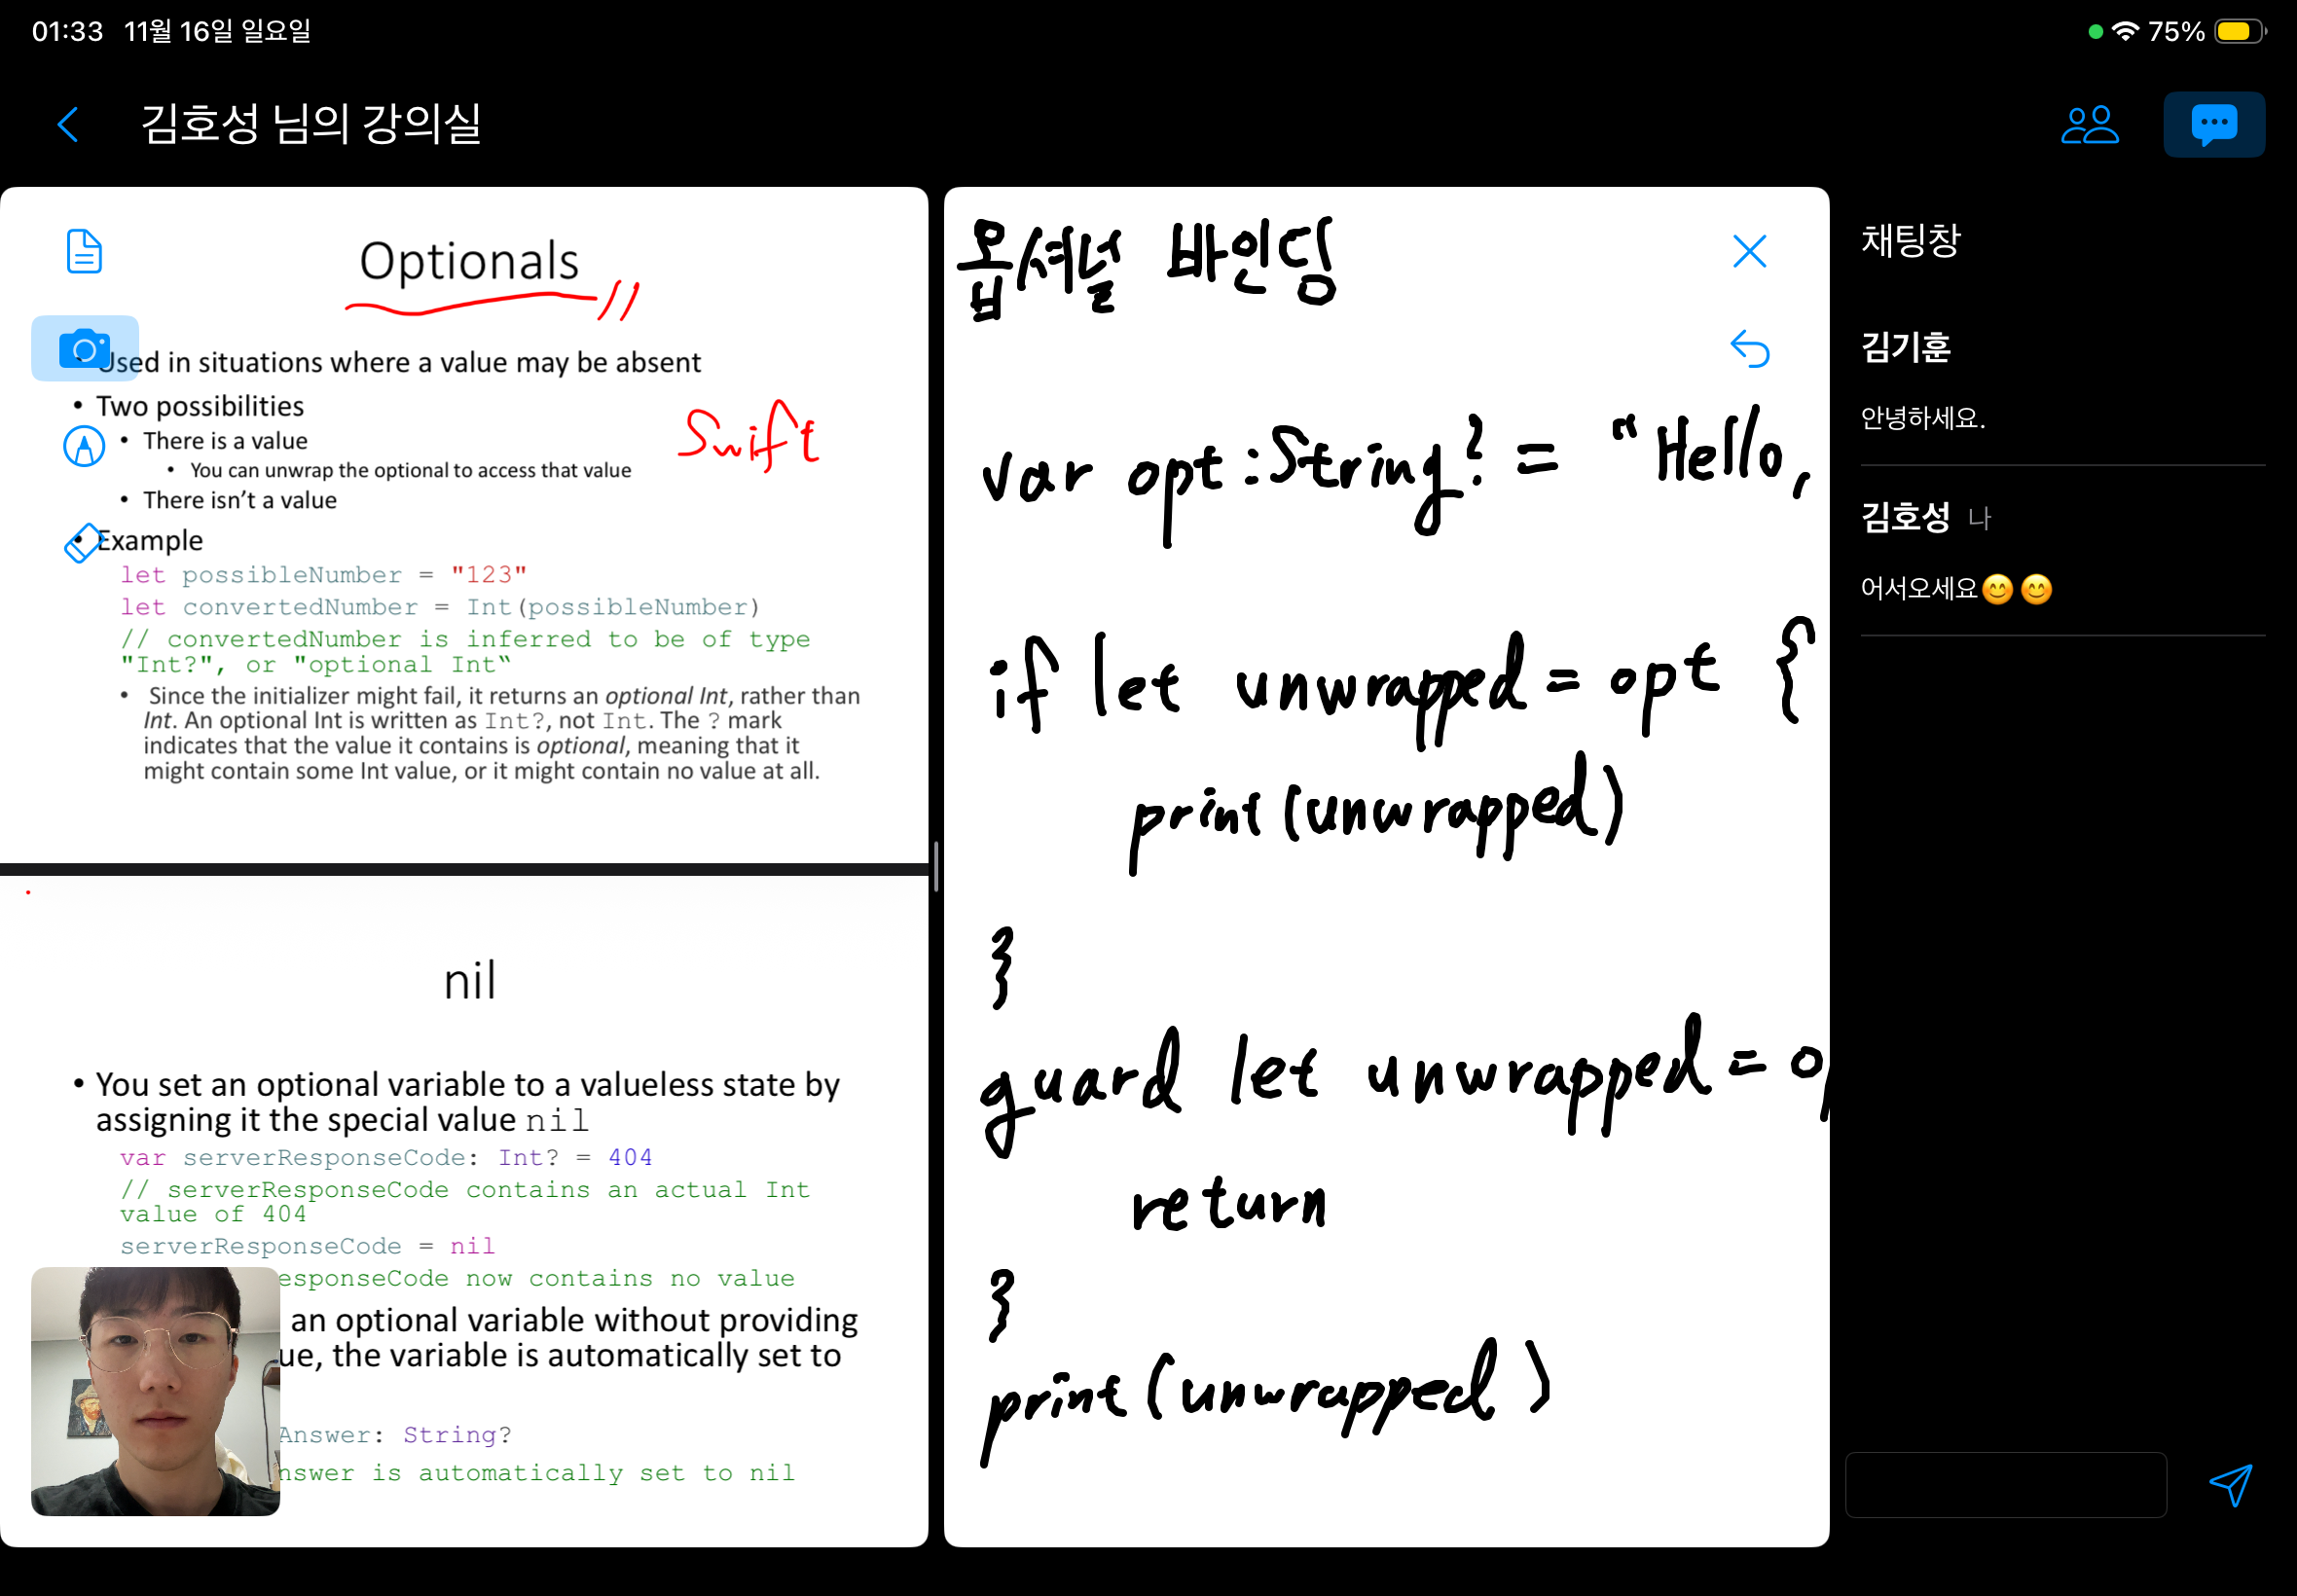
\includegraphics[width=0.9\textwidth]{fig5.png}
%\caption{User interface of a classroom screen with participants panel hidden}\label{fig5}
%\end{figure}
%
%\begin{figure}[H]
%\centering
%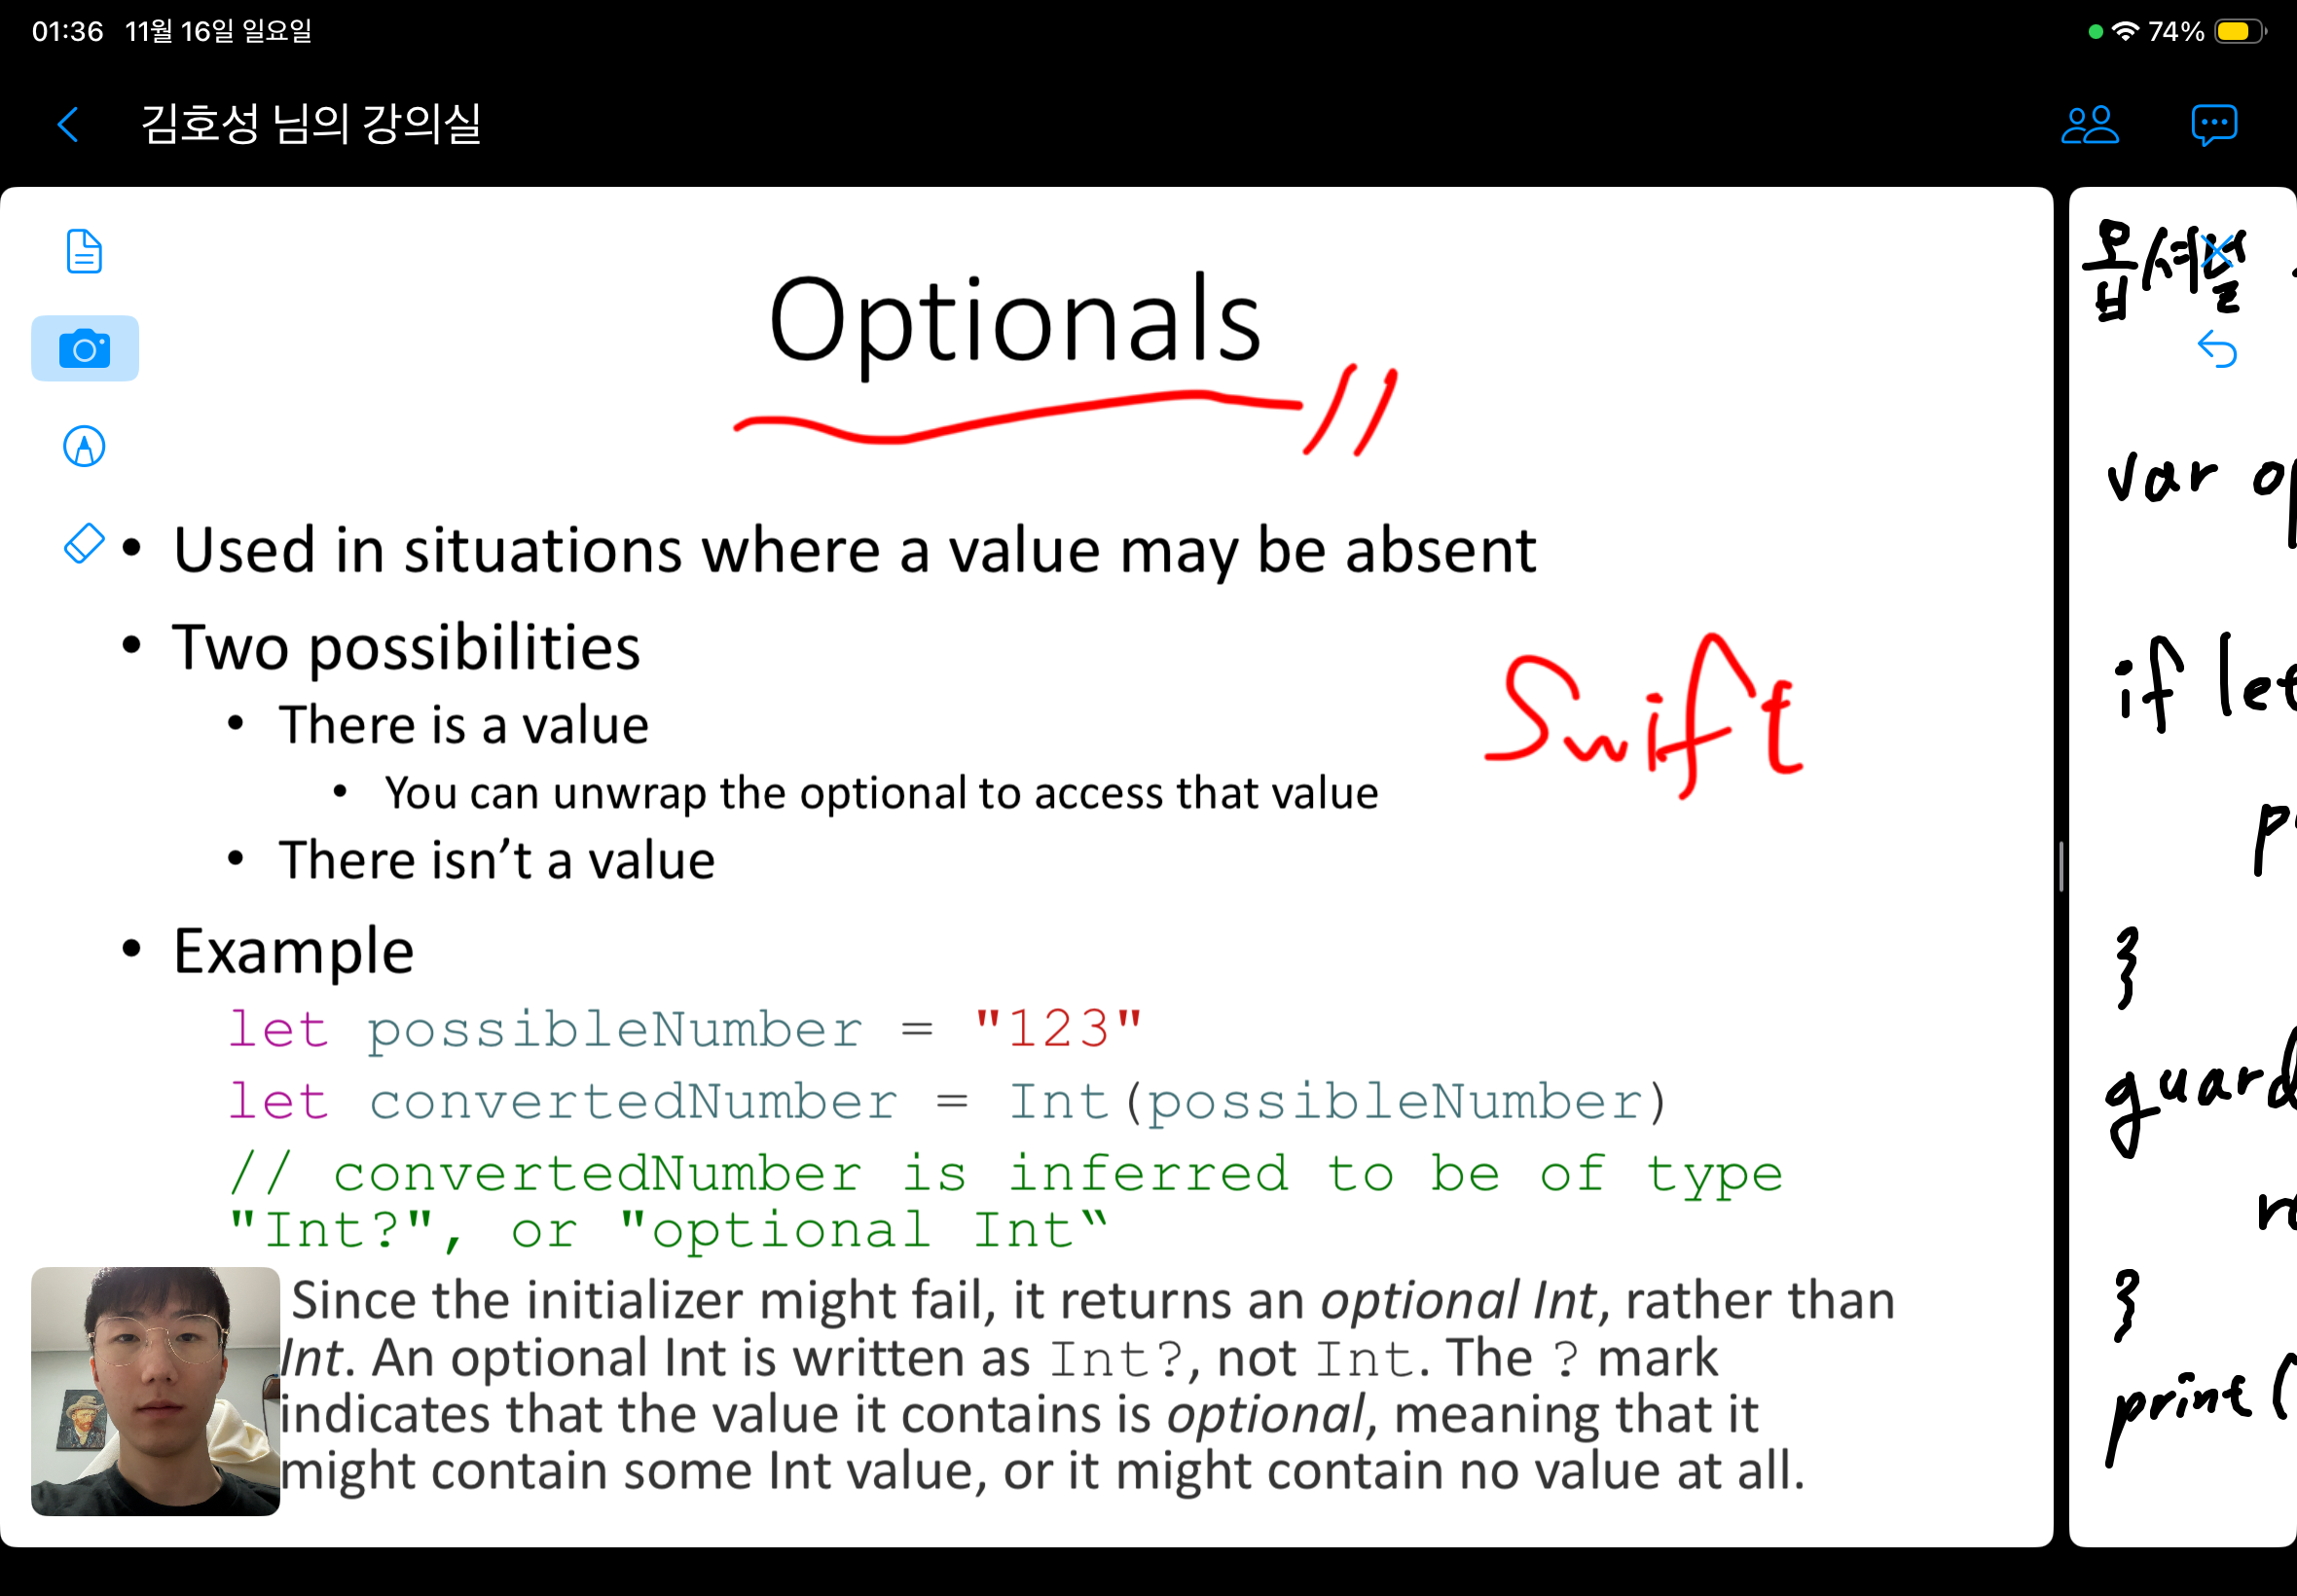
\includegraphics[width=0.9\textwidth]{fig6.png}
%\caption{User interface of a classroom screen with participants and chat panels hidden}\label{fig6}
%\end{figure}
%
%% 화면 녹화는 Apple Framework인 ReplayKit\cite{ReplayKit}을 사용하였다. ReplayKit은 전체 화면의 녹화 영상만을 제공하지만, 불필요한 UI의 전송을 방지하고 핵심 콘텐츠만 송출하기 위해 녹화 영상에서 강의 슬라이드와 화이트보드 영역만을 잘라내어 사용하였다. 음성은 AVAudioEngine을 통해 AVAudioBuffer 형태로 가져왔다.
%\noindent
%Screen recording is implemented using ReplayKit\cite{ReplayKit}. Although ReplayKit provides full-screen recording, only the regions corresponding to the lecture slides and whiteboard are cropped and transmitted to avoid unnecessary UI elements and focus on essential content. Audio is captured as \verb+AVAudioBuffer+ using \verb+AVAudioEngine+.
%
%% 이렇게 가져온 영상과 음성은 \verb+StreamService+의 \verb+MediaMixer+에서 하나의 스트림으로 합성된다. 합성된 스트림의 송출은 HaishinKit.swift\cite{HaishinKit} 라이브러리를 기반으로 스트리밍 서버와 직접 RTMP 통신을 수행하는 RTMPService에 의해 이루어진다. RTMPService는 RTMPConnection을 통해 스트리밍 서버와의 연결을 수립하고, RTMPStream을 통해 송출과 수신을 한다. 이때, 서버에서 강의실 생성 시 부여한 UUID 기반의 고유한 키 값을 streamName으로 설정하여 알맞은 강의실에 연결해 송출과 수신을 수행한다.
%The captured video and audio streams are combined into a single stream using the \verb+MediaMixer+ of \verb+StreamService+. The combined stream is transmitted via RTMP using HaishinKit.swift\cite{HaishinKit}. The \verb+RTMPService+ establishes a connection to the streaming server through \verb+RTMPConnection+ and handles streaming via \verb+RTMPStream+. A unique UUID assigned at room creation is used as the stream name to ensure proper mapping between instructors and students.
%
%% 위 과정을 통해 RTMPService를 통해 강사의 화면과 음성은 실시간으로 송출되고, 학생들은 해당 강의실의 스트림을 수신할 수 있다. 이로써 강의 슬라이드와 화이트보드 두 핵심 콘텐츠를 학생에게 동시에 제공할 수 있는 기술적 기반이 마련되었다. 그러나 모바일 기기의 제한된 크기의 화면에서 두 핵심 콘텐츠가 과도하게 작아지지 않도록 하는 UI 설계가 필요하였다.
%Through this process, the instructor’s screen and audio are streamed in real time, enabling students to simultaneously view lecture slides and whiteboard content. However, due to the limited screen size of mobile devices, an appropriate UI design is required to prevent these two key contents from becoming too small.
%
%% 따라서 강의자가 상황에 맞게 두 콘텐츠 영역의 크기를 조절할 수 있는 User-Adjustable UI를 적용하였다. 그림\ref{fig7}, \ref{fig8}과 같이 강의자는 grabber를 드래그하여 강의 슬라이드와 화이트보드의 화면 비율을 자유롭게 조절하며 강의 상황에 따라 필요한 정보를 유연하게 강조할 수 있다.
%To address this issue, a user-adjustable UI is introduced. As shown in Figures~\ref{fig7} and~\ref{fig8}, instructors can dynamically adjust the relative sizes of the slide and whiteboard areas by dragging a grabber. This allows flexible emphasis on different types of content depending on the lecture context.
%
%\begin{figure}[H]
%\centering
%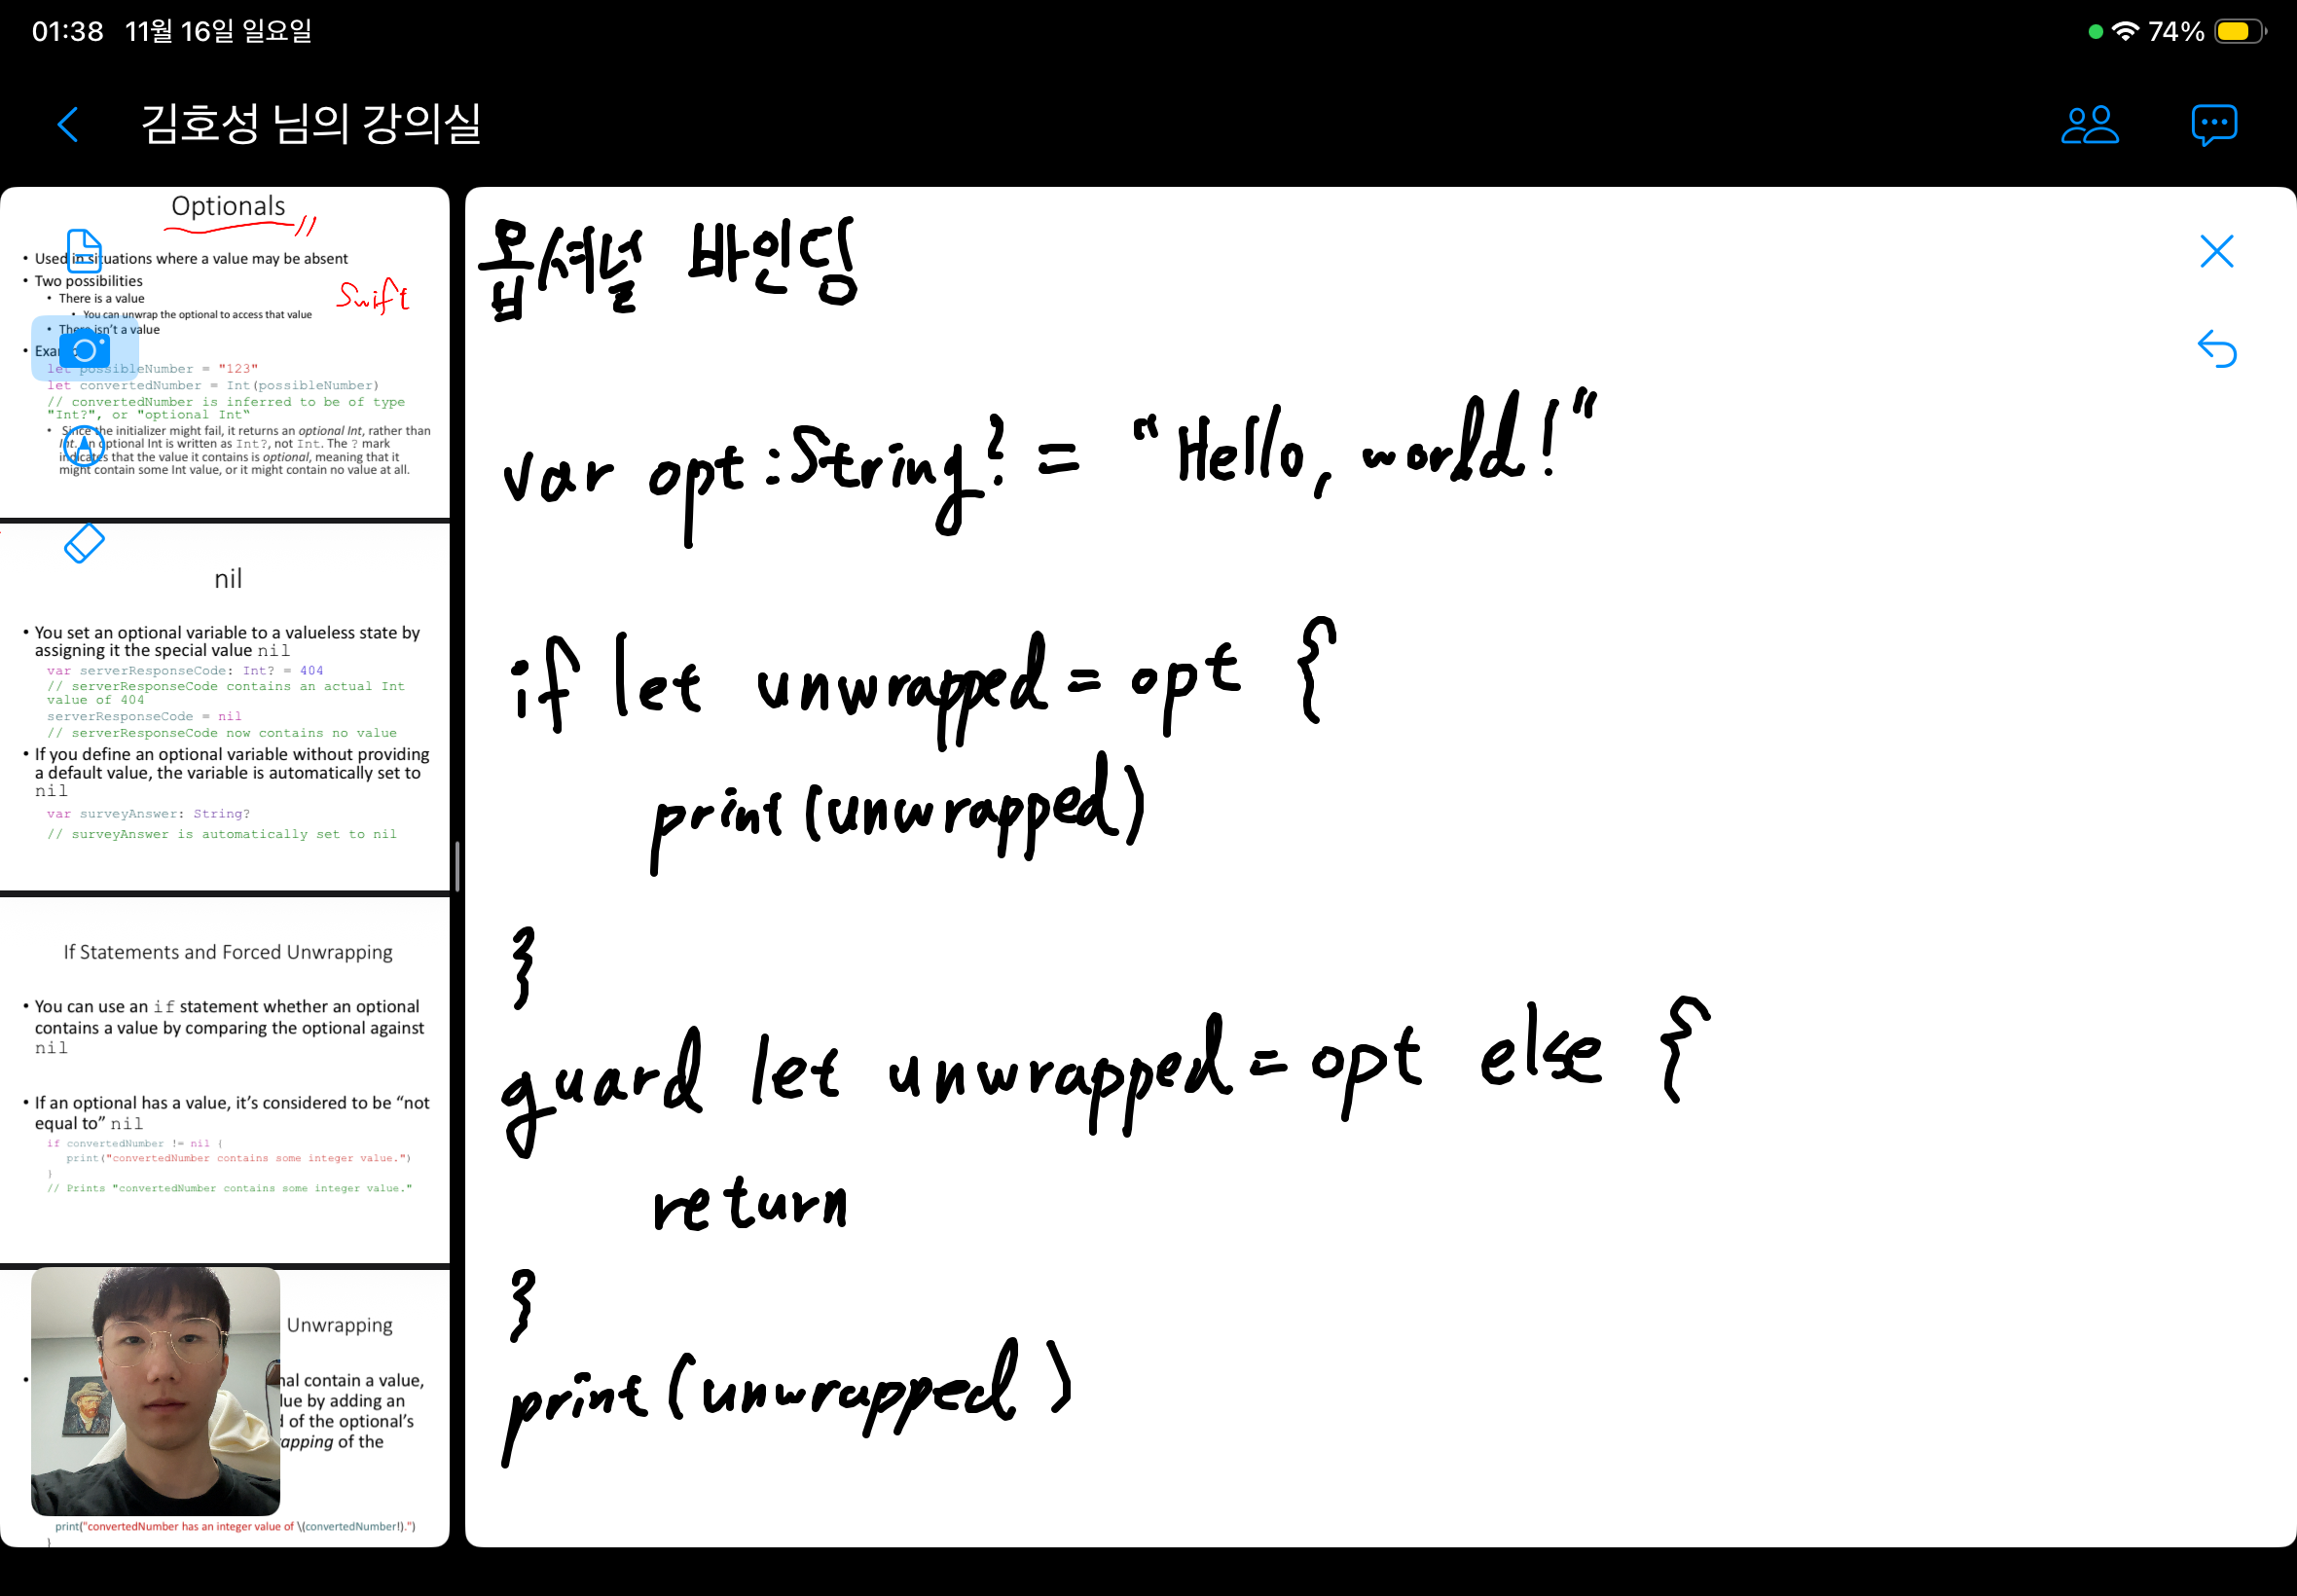
\includegraphics[width=0.9\textwidth]{fig7.png}
%\caption{User interface with an expanded lecture slide area}\label{fig7}
%\end{figure}
%
%\begin{figure}[H]
%\centering
%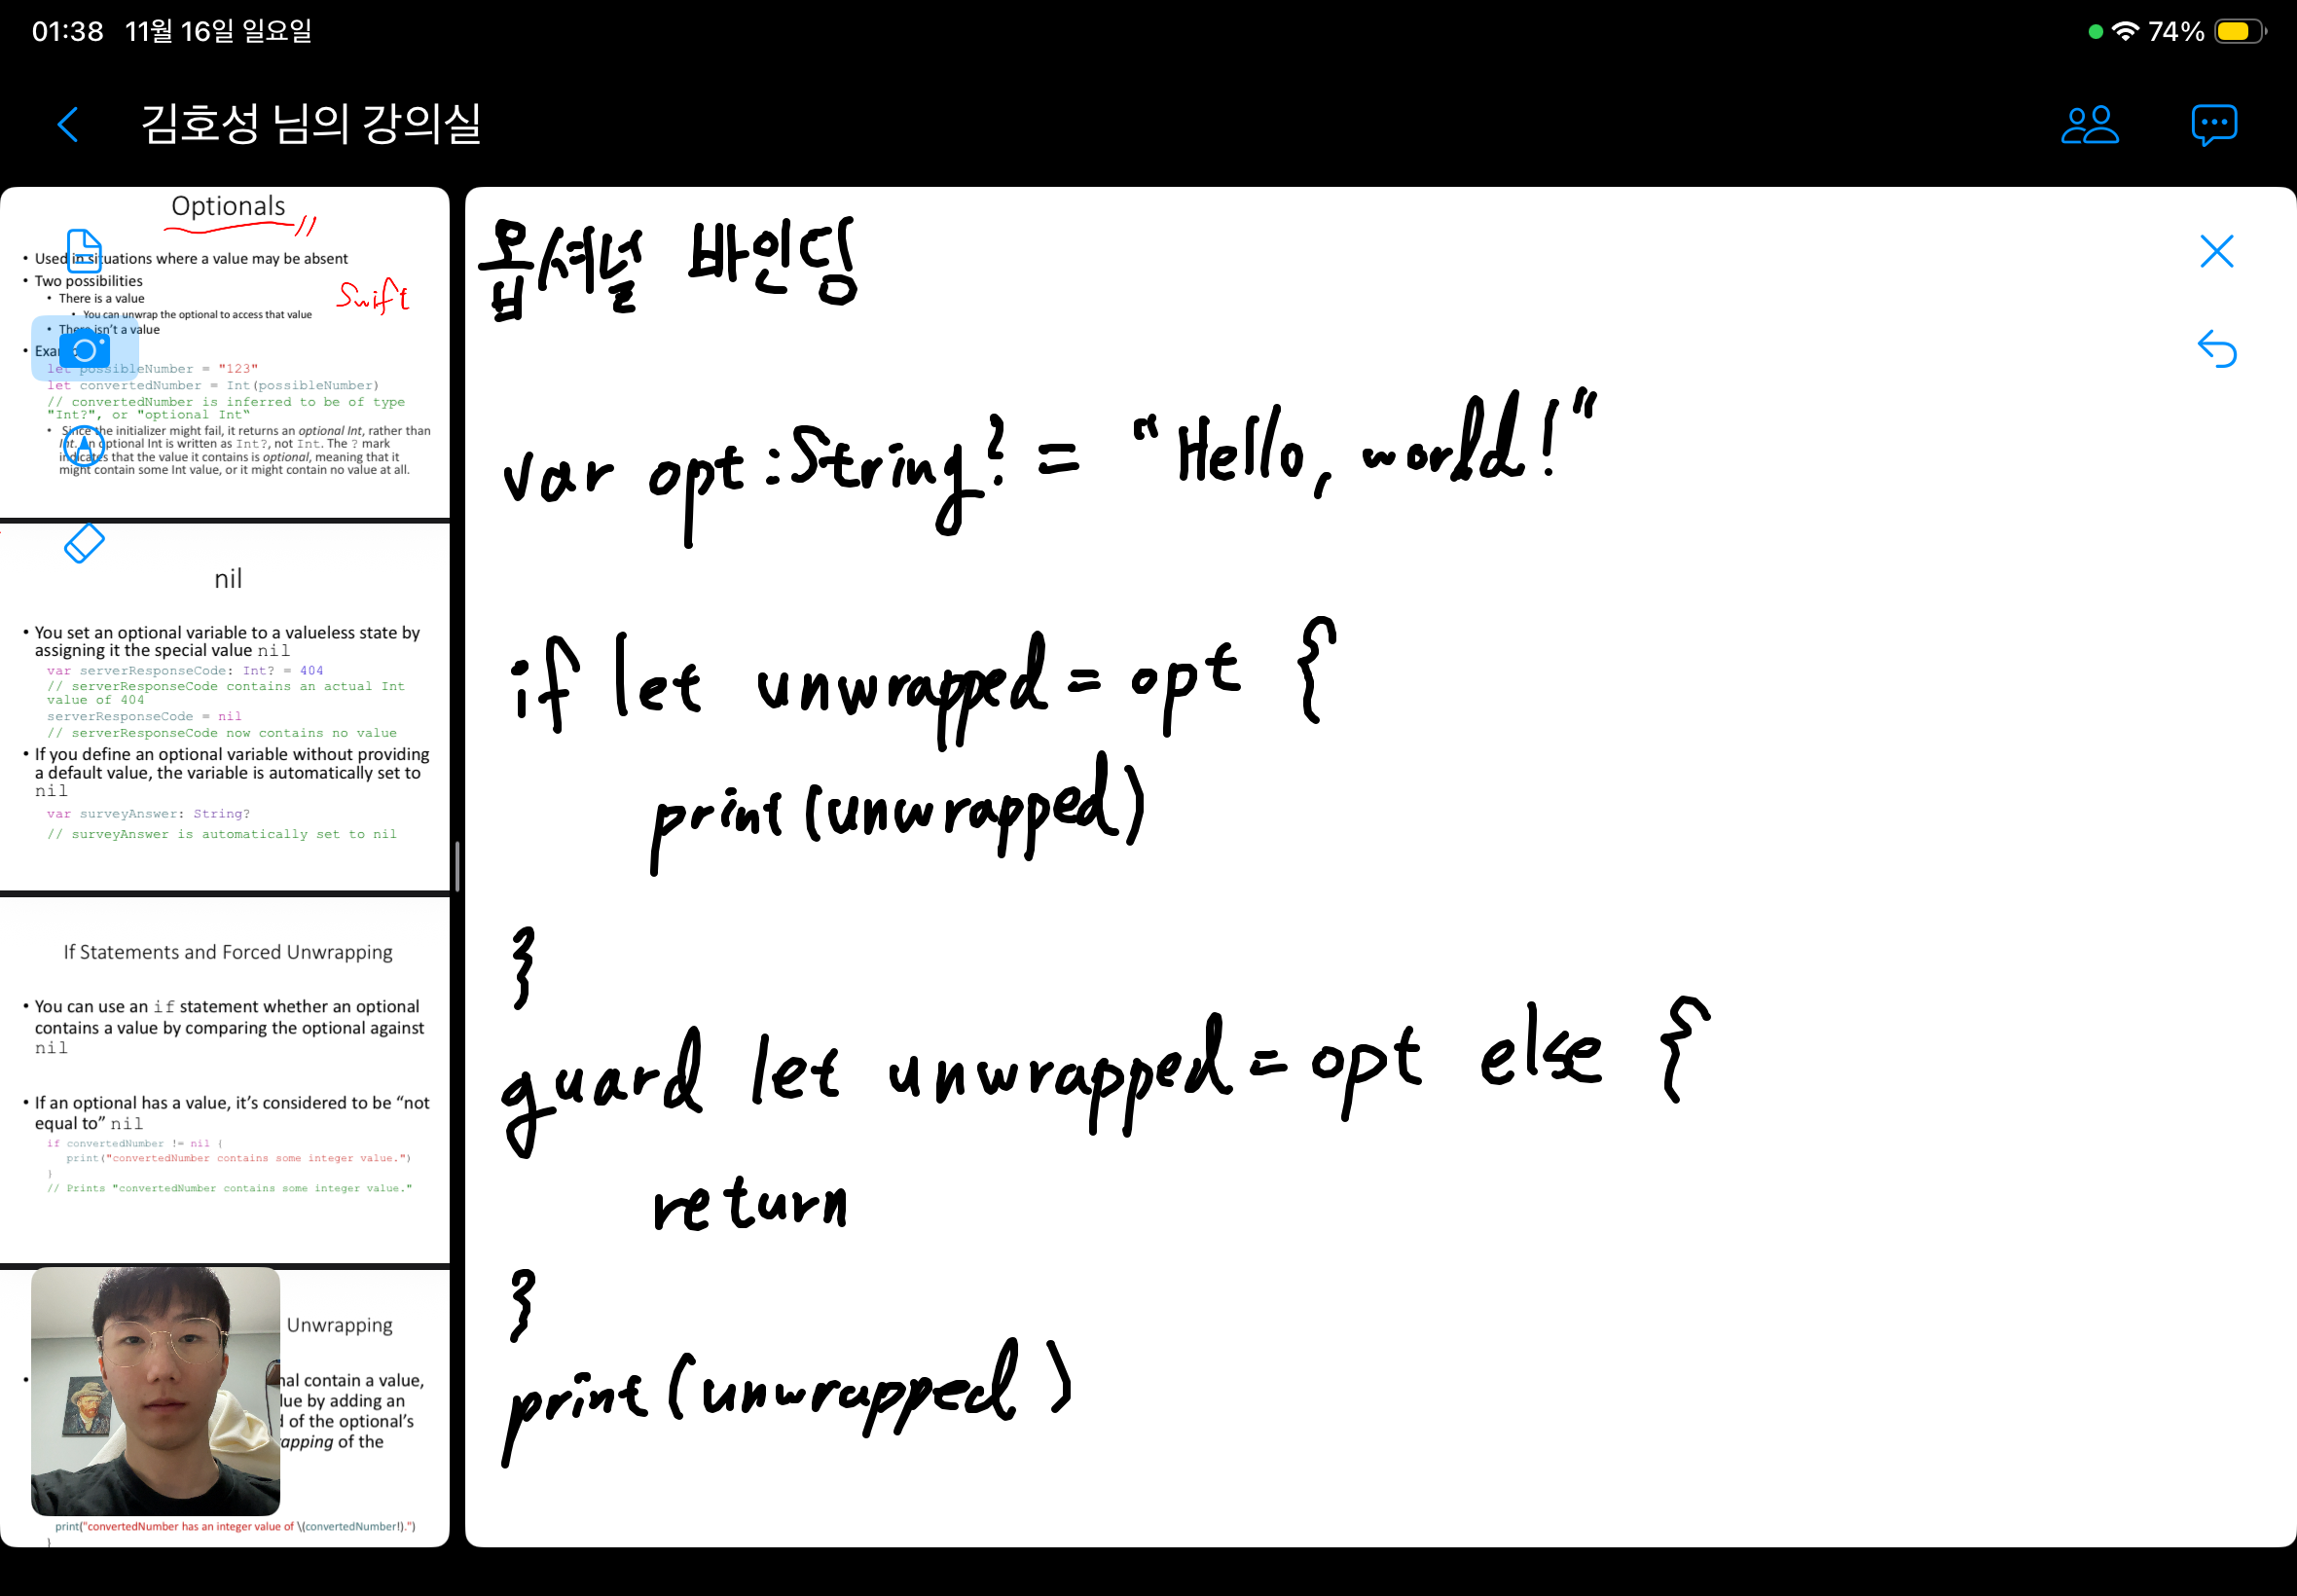
\includegraphics[width=0.9\textwidth]{fig8.png}
%\caption{User interface with an expanded whiteboard area}\label{fig8}
%\end{figure}
%
%% grabber는 \verb+UISlider+를 기반으로 구현되었으며, 사용자의 조작으로 value가 변경되면 \verb+valueChanged+ 이벤트를 통해 강의 슬라이드와 공유 화이트보드 화면 비율을 결정하는 \verb+NSLayoutConstraint+의 \verb+multiplier+값에 해당 값을 반영하였다. \verb+UISlider+는 투명하게 설정하여 화면에 드러나지 않고 로직적인 역할만을 수행하도록 하였다.
%\noindent
%The grabber is implemented based on a \verb+UISlider+. When the slider value changes, the \verb+valueChanged+ event updates the \verb+multiplier+ of the \verb+NSLayoutConstraint+ that determines the layout ratio between the slide and whiteboard views. The slider itself is visually hidden, serving only as a logical control element.

\section{Preliminary Evaluation}

% 제시된 시스템의 학습 지원 효과와 사용 편의성을 검증하기 위해 사용자 만족도 조사를 실시하였다. 평가는 총 5명을 대상으로 진행되었으며, 비교 대상 시스템은 강의 슬라이드와 화이트보드를 함께 배치하지 않고 둘 중 하나만 표시 가능한 Cisco Webex, 강의 슬라이드와 화이트보드가 5:5로 고정된 시스템, User-Adjustable UI를 적용한 시스템 위 세 가지였다.
% 각 시스템을 활용하여 강의를 진행한 후, 다음 세 질문에 대한 응답을 조사하였다. 첫째, 강의 슬라이드는 얼마나 잘 보였는가? 둘째, 화이트보드는 얼마나 잘 보였는가? 셋째, 강의 슬라이드와 화이트보드를 사용한 강의는 얼마나 이해하기 쉬웠는가? 각 항목에 대해 만족도에 따라 1점에서 5점을 평가하도록 하였으며, 그 결과는 아래의 표\ref{tab1}, \ref{tab2}, \ref{tab3}에서 확인할 수 있다.
% 표\ref{tab1}과 \ref{tab2}는 각각 `강의 슬라이드는 얼마나 잘 보였는가?'와 `화이트보드는 얼마나 잘 보였는가?'에 대한 응답 결과이다. Webex는 두 평가항목에서 모두 높은 점수를 받아, 강의 슬라이드나 화이트보드 둘 중 하나만 표시하는 것이 학습자의 가독성을 충분히 보장하였음을 확인할 수 있다. 반면 5:5 고정 UI 시스템은 슬라이드와 화이트보드를 동시에 제공하기 위해 두 영역이 작은 크기로 고정되어, 다른 두 시스템에 비해 유의미하게 낮은 평가를 받았다. 한편 User-Adjustable UI 시스템은 두 평가항목에서 모두 높은 점수를 받아, Webex와 비교해도 가독성 면에서 차이가 없음을 확인할 수 있었다. 이는 상황에 따라 강의 슬라이드나 화이트보드 영역을 확장할 수 있는 점이 학습자의 가독성을 충분히 확보할 수 있었다고 해석된다.

% To evaluate the learning effectiveness and usability of the proposed system, a user satisfaction survey was conducted with five participants.
To evaluate the effectiveness of the proposed system in supporting learning and its usability, a user satisfaction study was conducted. The evaluation involved five participants and compared three systems: (1) Cisco Webex, which allows only one of either lecture slides or a whiteboard to be displayed at a time, (2) a system with a fixed 5:5 split UI displaying both slides and a whiteboard simultaneously, and (3) the proposed system with a user-adjustable UI.

After conducting lectures using each system, participants were asked to respond to the following three questions: (1) How clearly visible were the lecture slides? (2) How clearly visible was the whiteboard? and (3) How easy was it to understand the lecture when both slides and the whiteboard were used? Each question was rated on a 5-point Likert scale, where 1 indicates very poor and 5 indicates excellent. The results are summarized in Tables \ref{tab1}, \ref{tab2}, and \ref{tab3}.

Tables \ref{tab1} and \ref{tab2} present the results for slide visibility and whiteboard visibility, respectively. Webex received consistently high scores in both categories, indicating that displaying only one content element at a time ensures sufficient readability. In contrast, the fixed 5:5 UI system received significantly lower scores, as both the slide and whiteboard areas were constrained to smaller sizes in order to be displayed simultaneously.

The proposed user-adjustable UI system achieved high scores in both categories, comparable to Webex. This suggests that allowing instructors to dynamically adjust the size of the slide and whiteboard areas effectively maintains readability for both types of content, depending on the lecture context.

\begin{table}
\caption{Respondents' perception of the visibility of a lecture slide}\label{tab1}
\begin{tabular*}{\textwidth}{@{\extracolsep\fill}lcccccc}
\toprule%
Target System & \multicolumn{5}{@{}c@{}}{Respondents} & Average\\\cmidrule{2-6}
& A & B & C & D & E &\\
\midrule
Webex  & 5 & 5 & 5 & 5 & 5 & 5 \\
5:5 Fixed UI  & 1 & 5 & 1 & 2 & 4 & 2.6 \\
User-Adjustable UI  & 5 & 5 & 5 & 5 & 5 & 5 \\
\bottomrule
\end{tabular*}
\end{table}

\begin{table}
\caption{Respondents' perception of the visibility of a whiteboard}\label{tab2}
\begin{tabular*}{\textwidth}{@{\extracolsep\fill}lcccccc}
\toprule%
Target System & \multicolumn{5}{@{}c@{}}{Respondents} & Average\\\cmidrule{2-6}
& A & B & C & D & E &\\
\midrule
Webex  & 3 & 5 & 5 & 4 & 4 & 4.2 \\
5:5 Fixed UI  & 1 & 3 & 2 & 3 & 5 & 2.8 \\
User-Adjustable UI  & 5 & 4 & 4 & 5 & 5 & 4.6 \\
\bottomrule
\end{tabular*}
\end{table}

% \noindent
% 표\ref{tab3}은 `강의 슬라이드와 화이트보드를 사용한 강의는 얼마나 이해하기 쉬웠는가?'에 대한 응답 결과이다. Webex는 평균 4.0점으로 긍정적인 평가를 받았지만 화이트보드를 사용하기 위해 강의 슬라이드를 종료해야 하는 제약으로 인해 약간의 감점을 받았다. 5:5 고정 UI 시스템은 평균 2.4점으로 가장 낮았는데, 많은 응답자들이 작은 크기의 강의 슬라이드로 인한 학습 경험 저하를 이유로 꼽았다. 반면, User-Adjustable UI 시스템은 평균 4.6점으로 가장 높은 점수를 받았는데, 이는 강의 슬라이드를 확장하여 강의 슬라이드 위주로 수업을 진행하거나 화이트보드를 확장하여 판서를 진행하는 등 상황에 맞는 활용이 가능하여 강의 이해도를 높일 수 있었기 때문이다.
Table \ref{tab3} presents the results for lecture comprehensibility when both slides and the whiteboard are used together. Webex received a relatively high average score of 4.0; however, some participants reported inconvenience due to the inability to use slides and the whiteboard simultaneously, resulting in a slight reduction in score. The fixed 5:5 UI system received the lowest average score of 2.4, with participants citing reduced readability of slides as a major factor negatively affecting their learning experience.

In contrast, the proposed system achieved the highest average score of 4.6. Participants noted that the ability to dynamically adjust the relative sizes of the slide and whiteboard allowed them to focus on the most relevant content at any given moment. For example, slides could be enlarged during explanation-heavy segments, while the whiteboard could be expanded during problem-solving or annotation phases. This flexibility contributed to improved overall lecture comprehension.

\begin{table}
\caption{Respondents' perception of the comprehensibility of a lecture with a lecture slide and a whiteboard combined}\label{tab3}
\begin{tabular*}{\textwidth}{@{\extracolsep\fill}lcccccc}
\toprule%
Target System & \multicolumn{5}{@{}c@{}}{Respondents} & Average\\\cmidrule{2-6}
& A & B & C & D & E &\\
\midrule
Webex  & 5 & 5 & 3 & 4 & 3 & 4 \\
5:5 Fixed UI  & 3 & 2 & 2 & 1 & 4 & 2.4 \\
User-Adjustable UI  & 4 & 4 & 5 & 5 & 5 & 4.6 \\
\bottomrule
\end{tabular*}
\end{table}

% \noindent
% 세가지 시스템에 대한 만족도 조사 결과를 종합하면, 본 보고서에서 제시한 User-Adjustable UI 시스템은 기존 원격 교육 시스템(Webex)과 단순 병렬 제공하는 5:5 고정 UI 시스템에 비해 전반적으로 높은 사용자 만족도를 보였다. Webex는 강의 슬라이드를 크게 제공한다는 장점이 있으나 화이트보드와 동시에 활용하지 못한다는 한계가 있었고, 5:5 고정 UI 시스템은 강의 슬라이드와 화이트보드를 동시에 사용할 수 있으나 각 요소가 지나치게 작아 학습 효과가 저하되는 문제가 있었다. 반면, 본 보고서에서 제시된 User-Adjustable UI 시스템은 이 두 시스템의 상반된 한계를 보완하여 강의 슬라이드와 화이트보드를 동시에 충분한 크기로 제공할 수 있다는 점에서 효과적인 대안임이 확인되었다.
Overall, the results demonstrate that the proposed user-adjustable UI system provides higher user satisfaction compared to both the conventional remote learning system (Webex) and the fixed 5:5 UI system. While Webex ensures high readability by displaying a single content type, it lacks the ability to present slides and whiteboard content simultaneously. On the other hand, the fixed 5:5 UI system enables simultaneous display but suffers from reduced readability due to limited screen space.

The proposed system effectively addresses these limitations by enabling both simultaneous presentation and flexible resizing of content. As a result, it provides an effective balance between visibility and functionality, leading to an improved learning experience on mobile devices.

\section{Conclusion}
% 본 보고서에서는 강의 슬라이드와 화이트보드를 동시에 시각적으로 제공하지 못하는 기존 시스템의 한계를 해결하기 위해 User-Adjustable UI 기반의 모바일 원격 교육 시스템을 설계 및 구현하였다. 제시된 시스템은 grabber를 통해 두 콘텐츠 영역의 비율을 상황에 맞게 조절할 수 있도록 하여, 제한된 크기의 모바일 기기 화면에서도 학습자가 필요한 정보를 충분한 크기로 확인할 수 있게 하였다. 또한 참여자 목록과 채팅창은 접이식 구조로 구현하여 불필요한 화면 점유를 최소화함으로써 제한된 화면 공간의 활용도를 높이고 학습 콘텐츠에 대한 시각적 집중을 강화하였다.
% 사용자 만족도 조사 결과, 제시된 시스템은 평가 항목인 강의 슬라이드의 가독성, 화이트보드의 가독성, 강의 이해도 세 측면에서 모두 다른 시스템보다 우수한 평가를 받아, User-Adjustable UI가 모바일 원격 교육 환경에서 학습 효과를 향상시키는 것을 확인하였다.
% 전체 소스코드는 \url{https://github.com/H0sungKim/CollaborativeComputingLab}에서 확인할 수 있다.
In this paper, we proposed and implemented a mobile distance learning system with a user-adjustable UI to address the limitation of existing systems that fail to effectively present both lecture slides and a whiteboard simultaneously. The proposed system allows instructors to dynamically control the relative sizes of these two content areas through a grabber interface, enabling learners to view essential information at an appropriate scale even on limited mobile screen sizes.

In addition, collapsible participant and chat panels were designed to minimize unnecessary screen occupancy, thereby improving the utilization of limited display space and enhancing visual focus on core learning content.

The results of the user satisfaction study demonstrate that the proposed system outperforms existing approaches in terms of slide visibility, whiteboard visibility, and overall lecture comprehension. These findings indicate that the user-adjustable UI effectively improves the learning experience in mobile distance learning environments.

The full source code of the proposed system is publicly available at: \\\url{https://github.com/H0sungKim/CollaborativeComputingLab}

\begin{credits}
\subsubsection{\ackname} Acknowledgements
\end{credits}
%
% ---- Bibliography ----
%
% BibTeX users should specify bibliography style 'splncs04'.
% References will then be sorted and formatted in the correct style.
%
% \bibliographystyle{splncs04}
% \bibliography{mybibliography}
%

\bibliographystyle{splncs04}
\bibliography{mybibliography}

\end{document}